\documentclass[times, utf8, zavrsni]{fer}
\usepackage{booktabs}
\usepackage[section]{placeins}
\usepackage{float}


\begin{document}

% TODO: Navedite broj rada.
\thesisnumber{5375}

% TODO: Navedite naslov rada.
\title{Programska podrška za svršenike}

% TODO: Navedite vaše ime i prezime.
\author{Tomislav Kravaršćan}

\maketitle

% Ispis stranice s napomenom o umetanju izvornika rada. Uklonite naredbu \izvornik ako želite izbaciti tu stranicu.
\izvornik

% Dodavanje zahvale ili prazne stranice. Ako ne želite dodati zahvalu, naredbu ostavite radi prazne stranice.
\zahvala{}

\tableofcontents

\chapter{Uvod}
Svršenici (lat. \textit{alumni}) je popularan naziv za bivše pripadnike neke ustanove, najčešće sveučilišta. Alumni su uobičajena udruženja u svijetu pa u nekim sveučilištima imaju i stoljetnu tradiciju. Njihovo ponovno okupljanje i sudjelovanje u radu sveučilišta je vrlo bitno za održavanje priče o prošlosti, a i za planiranje budućnosti sveučilišta. No, kako studenti sveučilišta vrlo brzo nakon diplomiranja utonu u nove životne prilike kao što su posao i obitelj, fakultetima je vrlo teško održavati vezu sa svojim bivšim studentima i ponovno ih okupljati. A i sami se svršenici teško održe na okupu. Za to je rješenje programska podrška u obliku društvene web aplikacije, gdje će se moći organizirati događaji, sastanci i objavljivati razne objave vezane za svršenike.

\chapter{Analiza postojeće programske podrške}
Analizom postojeće programske potpore nastojimo bolje razumijeti problem koji rješavamo, njegovu domenu primjene i razrješiti moguće krive početne pretpostavke o programskoj podršci koju izrađujemo. Također, jasnije vidimo funkcionalnosti koje bi trebali implementirati i dobivamo ideje o nekim detaljima o kojima uopće nismo razmišljali. Osim toga, svrha analize je i otrkivanje mogućih nedostataka koje trpi posojeća programska podrška, te učenje na tuđim pogreškama. Moramo biti posebno svjesni kojim su resursima raspolagali razvojni inženjeri analiziranih rješenja kako bismo što ranije odredili doseg našeg rješenja sukladno našim resursima vremena i znanja.
U ovom konkretnom slučaju, analizirati ćemo programska rješenja za upravljanje svršenicima. Takvih rješenja ima neiscrpno puno pa ćemo navesti samo neka od njih. Gotovo sva postojeća rješenja nude neke osnovne funkcionalnosti kao što su organizacija i pregled događaja, pregled novosti, informacije o sustavu, ponuda poslova, stvaranje i upravljanje korisničkim računom.

\section{Graduway}
Graduway[1] je web platforma istoimene tvrtke koja za različite fakultete po narudžbi stvara aplikaciju prilagođenu određenoj ustanovi za koju se izrađuje. Uz gore navedene osnovne funkcionalnosti ovakvog i sličnih rješenja, Graduway ima još puno funkcionalnosti kao što su adminske stranice, pregled statistike korisnika i vizualizacija itd. Dostupna je za isporuku na iOS, Android ili kao web- aplikacija.

Neki od njihovih klijenata za rješenje upravljanja svršenicima su Longwood University, University of Dundee, Brunel University, UCLA i mnogi drugi.

Svako rješenje je napravljeno za preko tisuću korisnika, početna cijena je pet tisuća dolara godišnje, te je ponuđen besplatni probni period.

\begin{figure}[H]
	\centering
	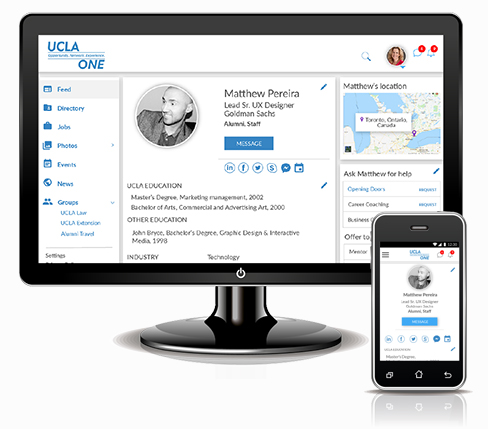
\includegraphics[width=13cm]{slike/izgledUCLAgraduwayRjesenja.png}
	\caption{Izgled UCLA Graduway rješenja}
	\label{fig:ucla-graduway}
\end{figure}

\section{VeryConnect}
VeryConnect je nešto manje popularna platforma za upravljanje svršenicima, ali sa jednako opširnim funkcionalnostima. Ima znatno manji broj klijenata od kojih je samo jedno sveučilište, University of Glasgow. Također ima neku početnu cijenu koja za razliku od Graduway-a nije javno vidljiva, a dodatne funkcionalnosti se naplaćuju zasebno.

\begin{figure}[H]
	\centering
	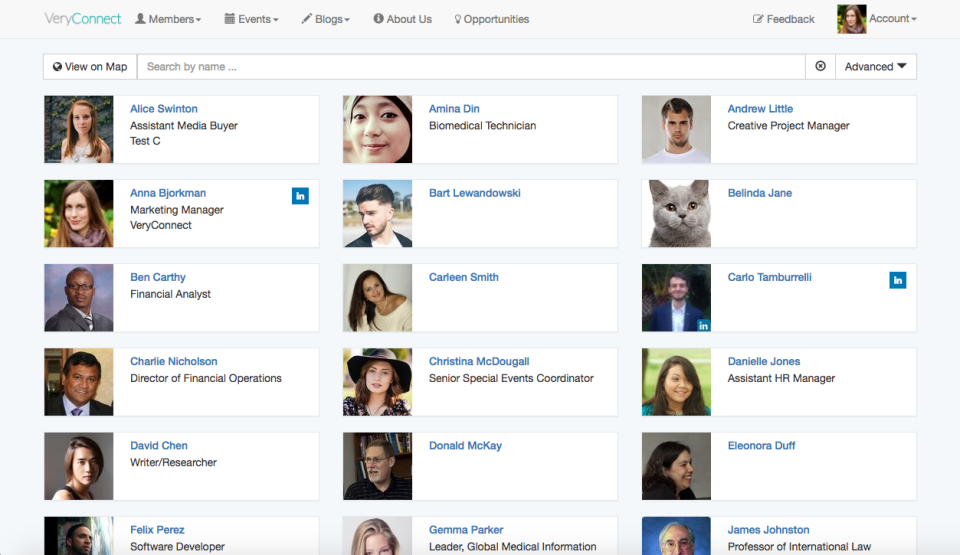
\includegraphics[width=13cm]{slike/very-connect-korisnici.png}
	\caption{VeryConnect - pregled korisnika}
	\label{fig:veryconn-users}
\end{figure}

\begin{figure}[H]
	\centering
	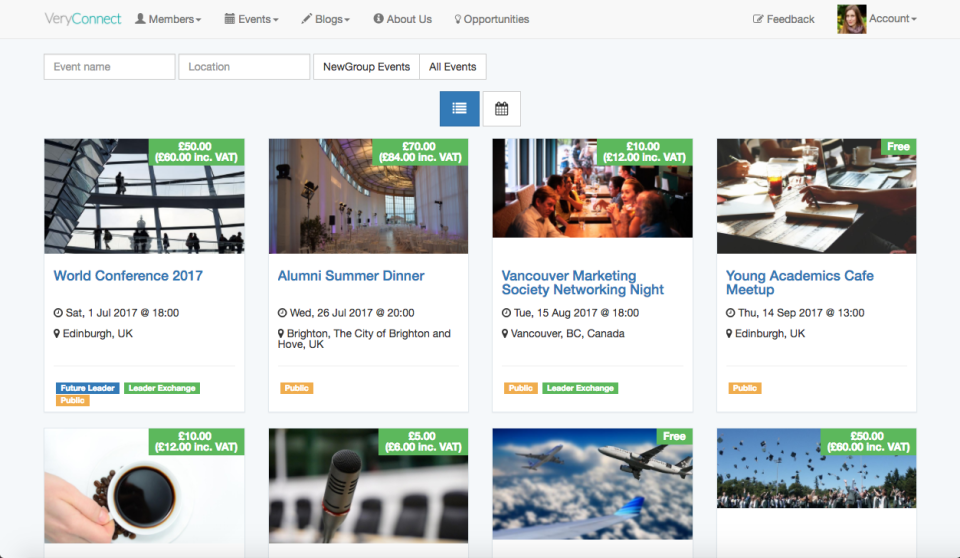
\includegraphics[width=13cm]{slike/very-connect-dogadaji.png}
	\caption{VeryConnect - pregled događaja}
	\label{fig:veryconn-events}
\end{figure}

\section{Hiverbrite}
Hiverbrite je također platforma sa vrlo opširnim funkcionalnostima.

\begin{figure}[H]
	\centering
	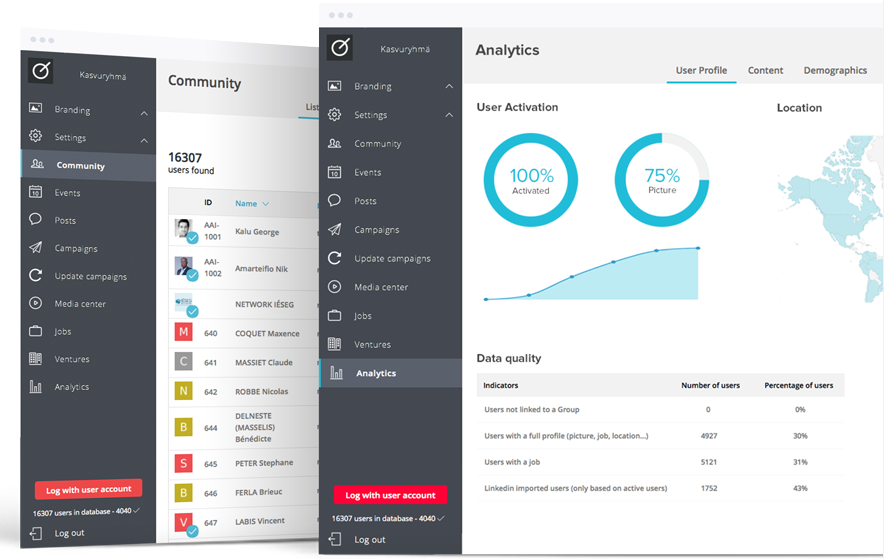
\includegraphics[width=13cm]{slike/hiverbrite-upravljanje.png}
	\caption{Izgled Hiverbrite stranice za upravljanje zajednicom}
	\label{fig:hiverbrite-menagements}
\end{figure}

\chapter{Zahtjevi nad programskom potporom}
Zahtjevi nad programskom potporom dijele se na funkcionalne zahtjeve – ono što korisnik očekuje od sustava i osnovne potrebe zbog kojih korisnik želi programsku potporu, te nefunkcionalne zahtjeve – ograničenja sustava i način na koji sustav treba biti izveden.

\section{Funkcionalni zahtjevi}
Funkcionalni zahtjevi su izjavljeni u prirodnom jeziku u obliku slučajeva korištenja, forma svakog slučaja korištenja: naziv slučaja korištenja – glavni sudionik.

 
\begin{itemize}
	\item Pregled postova - korisnik
	\item Pregled arhive postova - korisnik
	\item Filtriranje postova po kategoriji - korisnik
	\item Dodavanje posta - administrator
	\item Brisanje posta - administrator
	\item Uređivanje posta - administrator
	\item Pregled korisničkog računa - korisnik
	\item Dodavanje korisničkog računa (registracija) - anonimni korisnik
	\item Brisanje korisničkog računa - korisnik 
	\item Uređivanje korisničkog računa - korisnik
	\item Pregled svih korisnika - administrator
	\item Prijava na sustav - korisnik 
	\item Odjava sa sustava - korisnik
	\item Preplata na kategoriju - korisnik
	\item Otkazivanje pretplate na kategoriju - korisnik
	\item Slanje pošte obavijesti prilikom objave novog posta - aplikacija
\end{itemize}

\section{Nefunkcionalni zahtjevi}
Nefunkcionalni zahtjevi su sljedeći:

\begin{itemize}
	\item Sustav mora podržavati istodobni rad više korisnika
	\item Sustav mora biti otporan na kritične pogreške
	\item Sustav mora biti otporan na XSS ranjivosti
	\item Sustav mora biti ostvaren MVC arhitekturom kao web aplikacija
	\item Sustav mora biti u mogućnosti spremati podatke u bazu podataka
\end{itemize}

\chapter{Arhitektura sustava}
\section{Baza podataka}
\subsection{Konceptualni model baze podataka}

\subsection{Fizički model baze podataka}

\chapter{Implementirane funkcionalnosti}
Pregled funkcionalnosti koje posjeduje programska potpora. Svaka funkcionalnost je popraćena opisom i slikom koja pokazuje njenu implementaciju.

\section{Navigacijska traka}

\begin{figure}[H]
	\centering
	
\includegraphics[width=13cm]{slike/nav-admin.png}
	\caption{Navigacijska traka admistratora}
	\label{fig:nav-admin}
\end{figure}

Navigacijska traka je html element koji se pojavljuje u svim html stranicama aplikacije i svrha joj je omogućavanje dolaska do svih stranica aplikacije. Svaki korisnik putem navigacijske trake u svakom trenutku može doći do početne stranice, gdje je popis svih postova, odabirom "Alumni" natpisa u lijevom dijelu trake. 

\subsection{Navigacijska traka za anonimnog(ne prijavljenog) korisnika}
Anonimni korisnik pomoću navigacijske trake može doći do stranice za registraciju, stranice za prijavu te ima pregled svih poveznica koje su u sustavu. 

\subsection{Navigacijska traka za prijavljenog korisnika}
Prijavljenom se korisniku više ne prikazuje mogućnost odabira prijave niti registracije, nego u desnom dijelu trake ima prikaz svoga imena kojeg može odabrati. Tim odabirom mu se prikazuje padajući izbornik koji prikazuje dvije dodatne opcije, prikaz vlastitog profila, te odjava sa sustava.

Navigacijska traka je posebno bitna i administratoru sustava, koji, ako je prijavljen, vidi dodatnu opciju odabira padajućeg izbornika "Admin", čijim odabirom se otvara padajući izbornik sa opcijama izrade novog posta, pregleda arhive postova, svih korisnika, kategorija te poveznica.

\subsection{Registracija na sustav}

\begin{figure}[H]
	\centering
	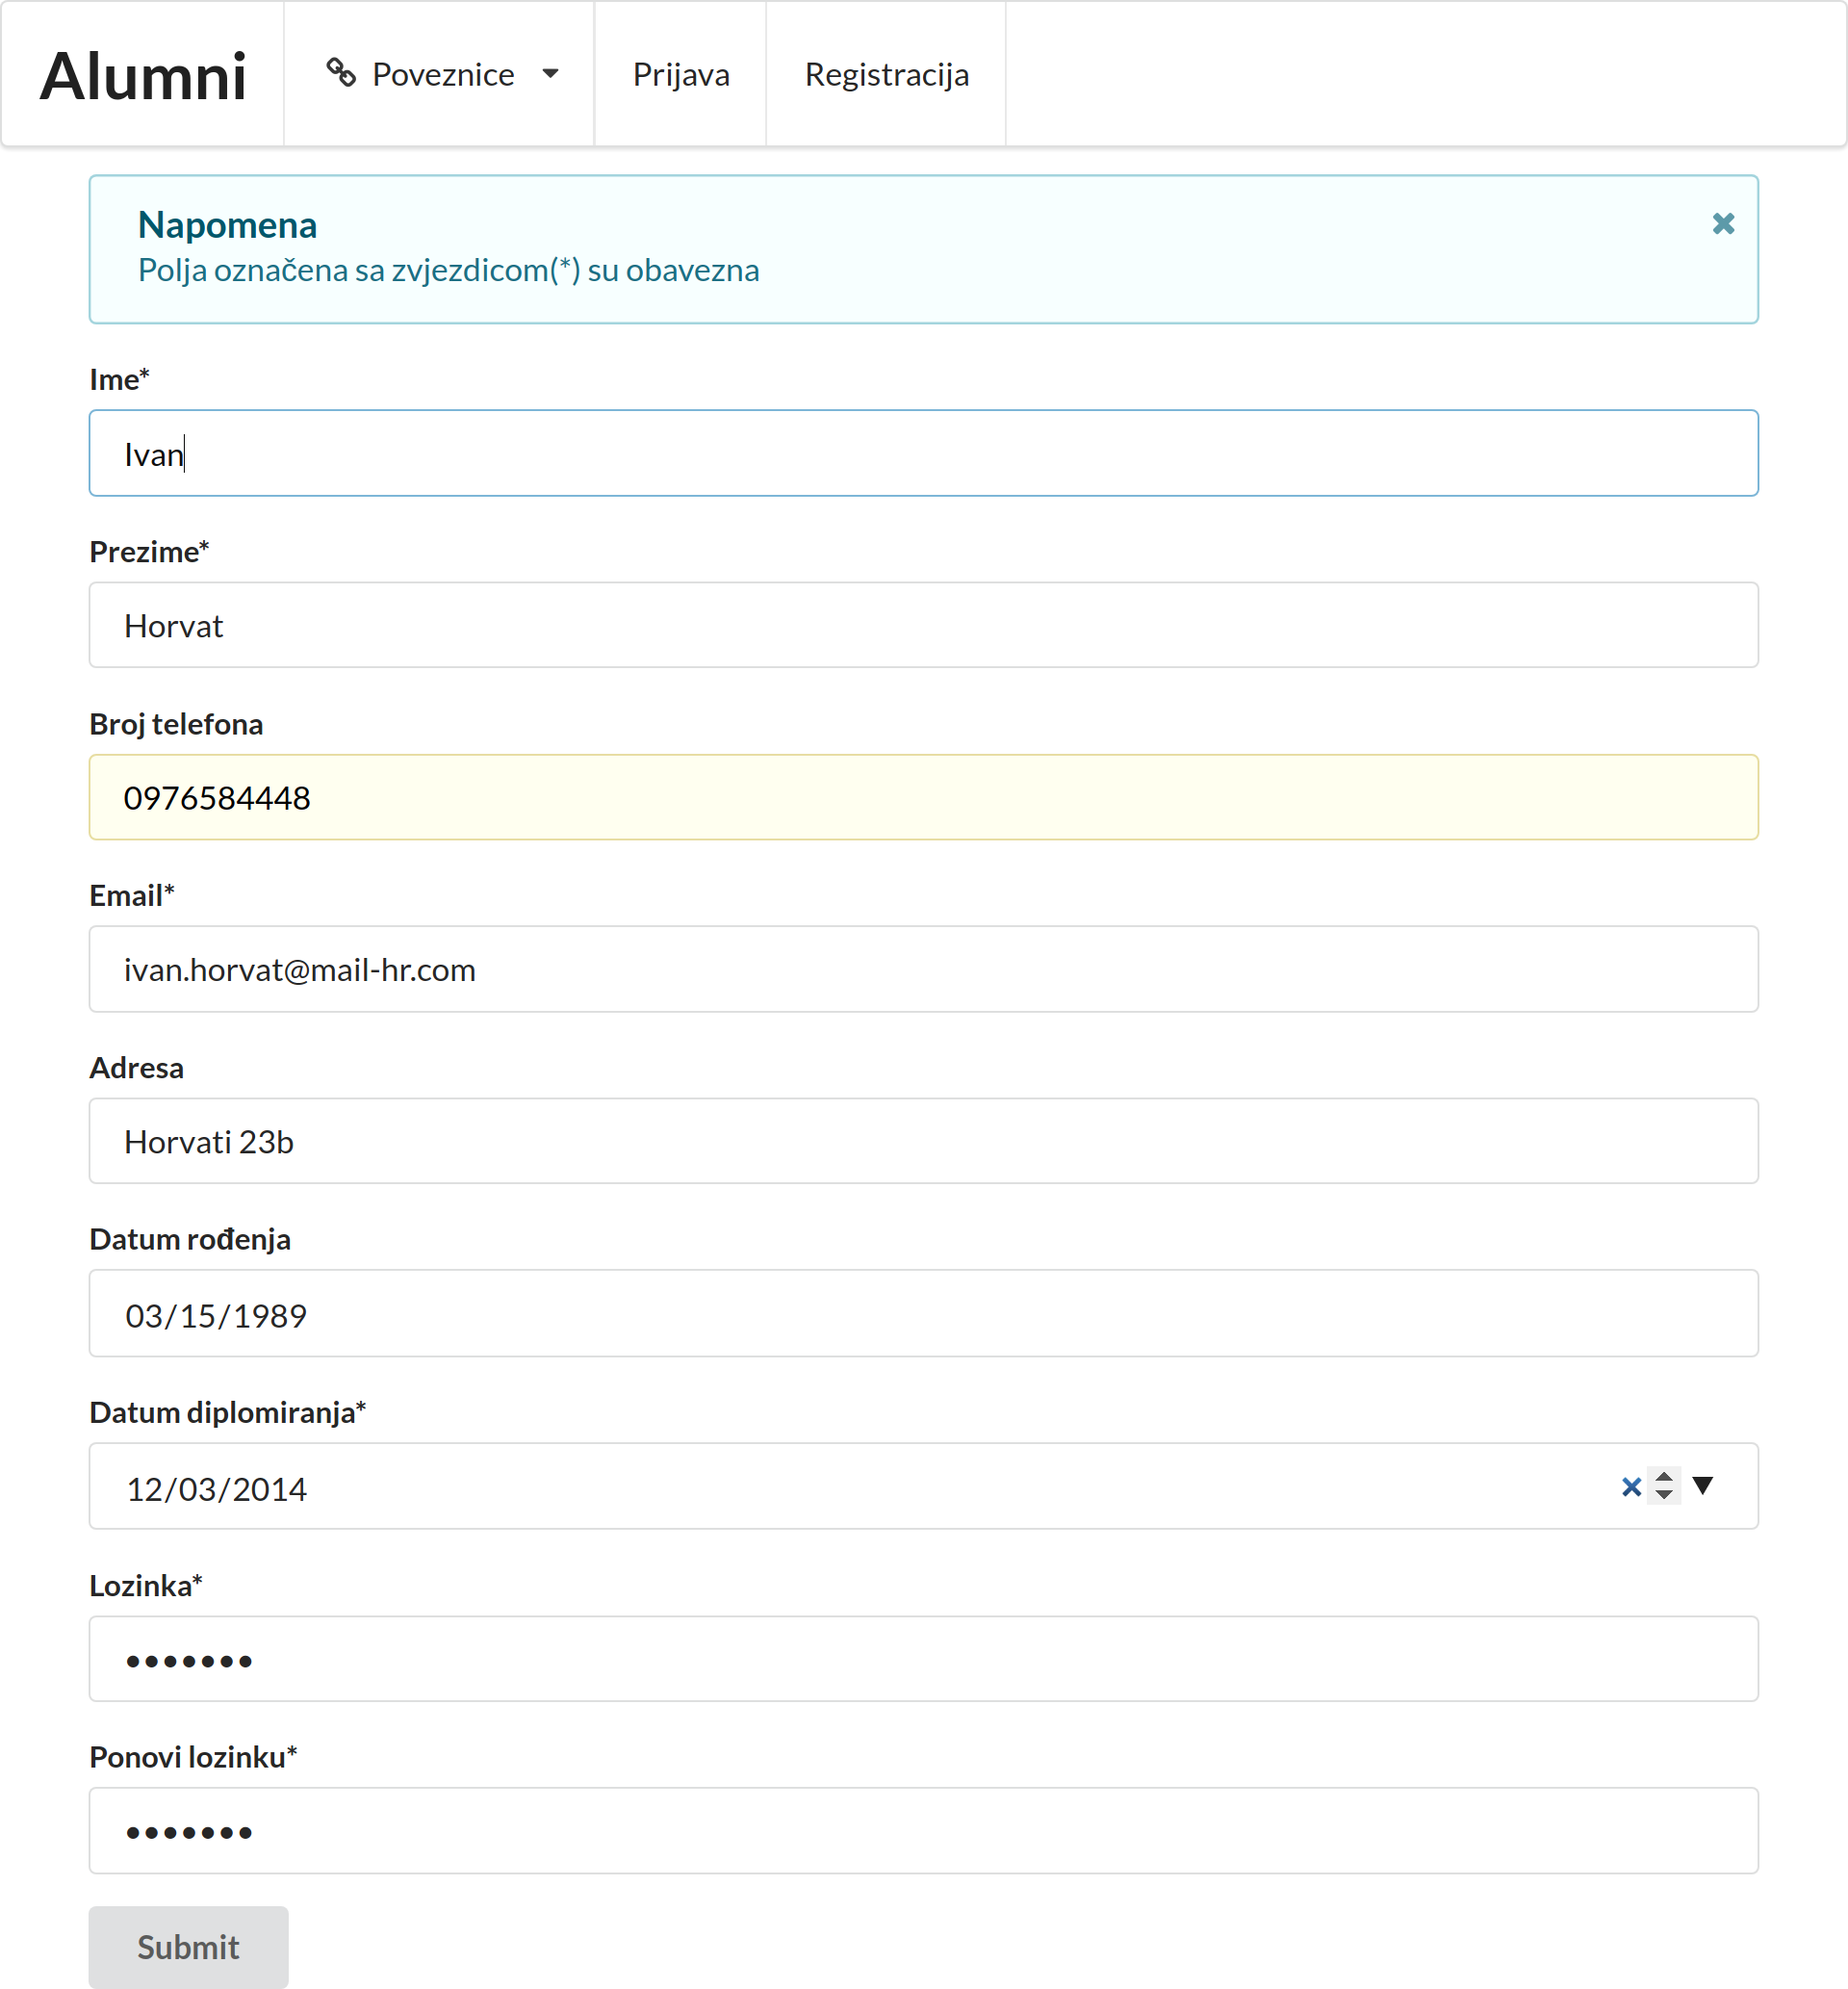
\includegraphics[width=13cm]{slike/registracija.png}
	\caption{Obrazac za registraciju}
	\label{fig:registracija}
\end{figure}

Prilikom odabira opcije "Registracija" u navigacijskoj traci, anonimnom se korisniku prikaže obrazac za registraciju na sustav. Kako bi se uspješno registrirao, korisnik mora upisati ime, prezime, email, datum diplomiranja te lozinku. Broj telefona, adresa i datum rođenja su neobavezna polja te se korisniku daje na izbor hoće li ih upisati ili ne. Za sve navedene obavezne stavke postoje provjere na klijentskoj te na poslužiteljskoj strani, te osim provjera za postojanost obaveznih stavki, postoje i provjere za ispravnost email-a, te provjere da li lozinka ima najmanje 6, a najviše 30 znakova.

\subsection{Prijava na sustav}

\begin{figure}[H]
	\centering
	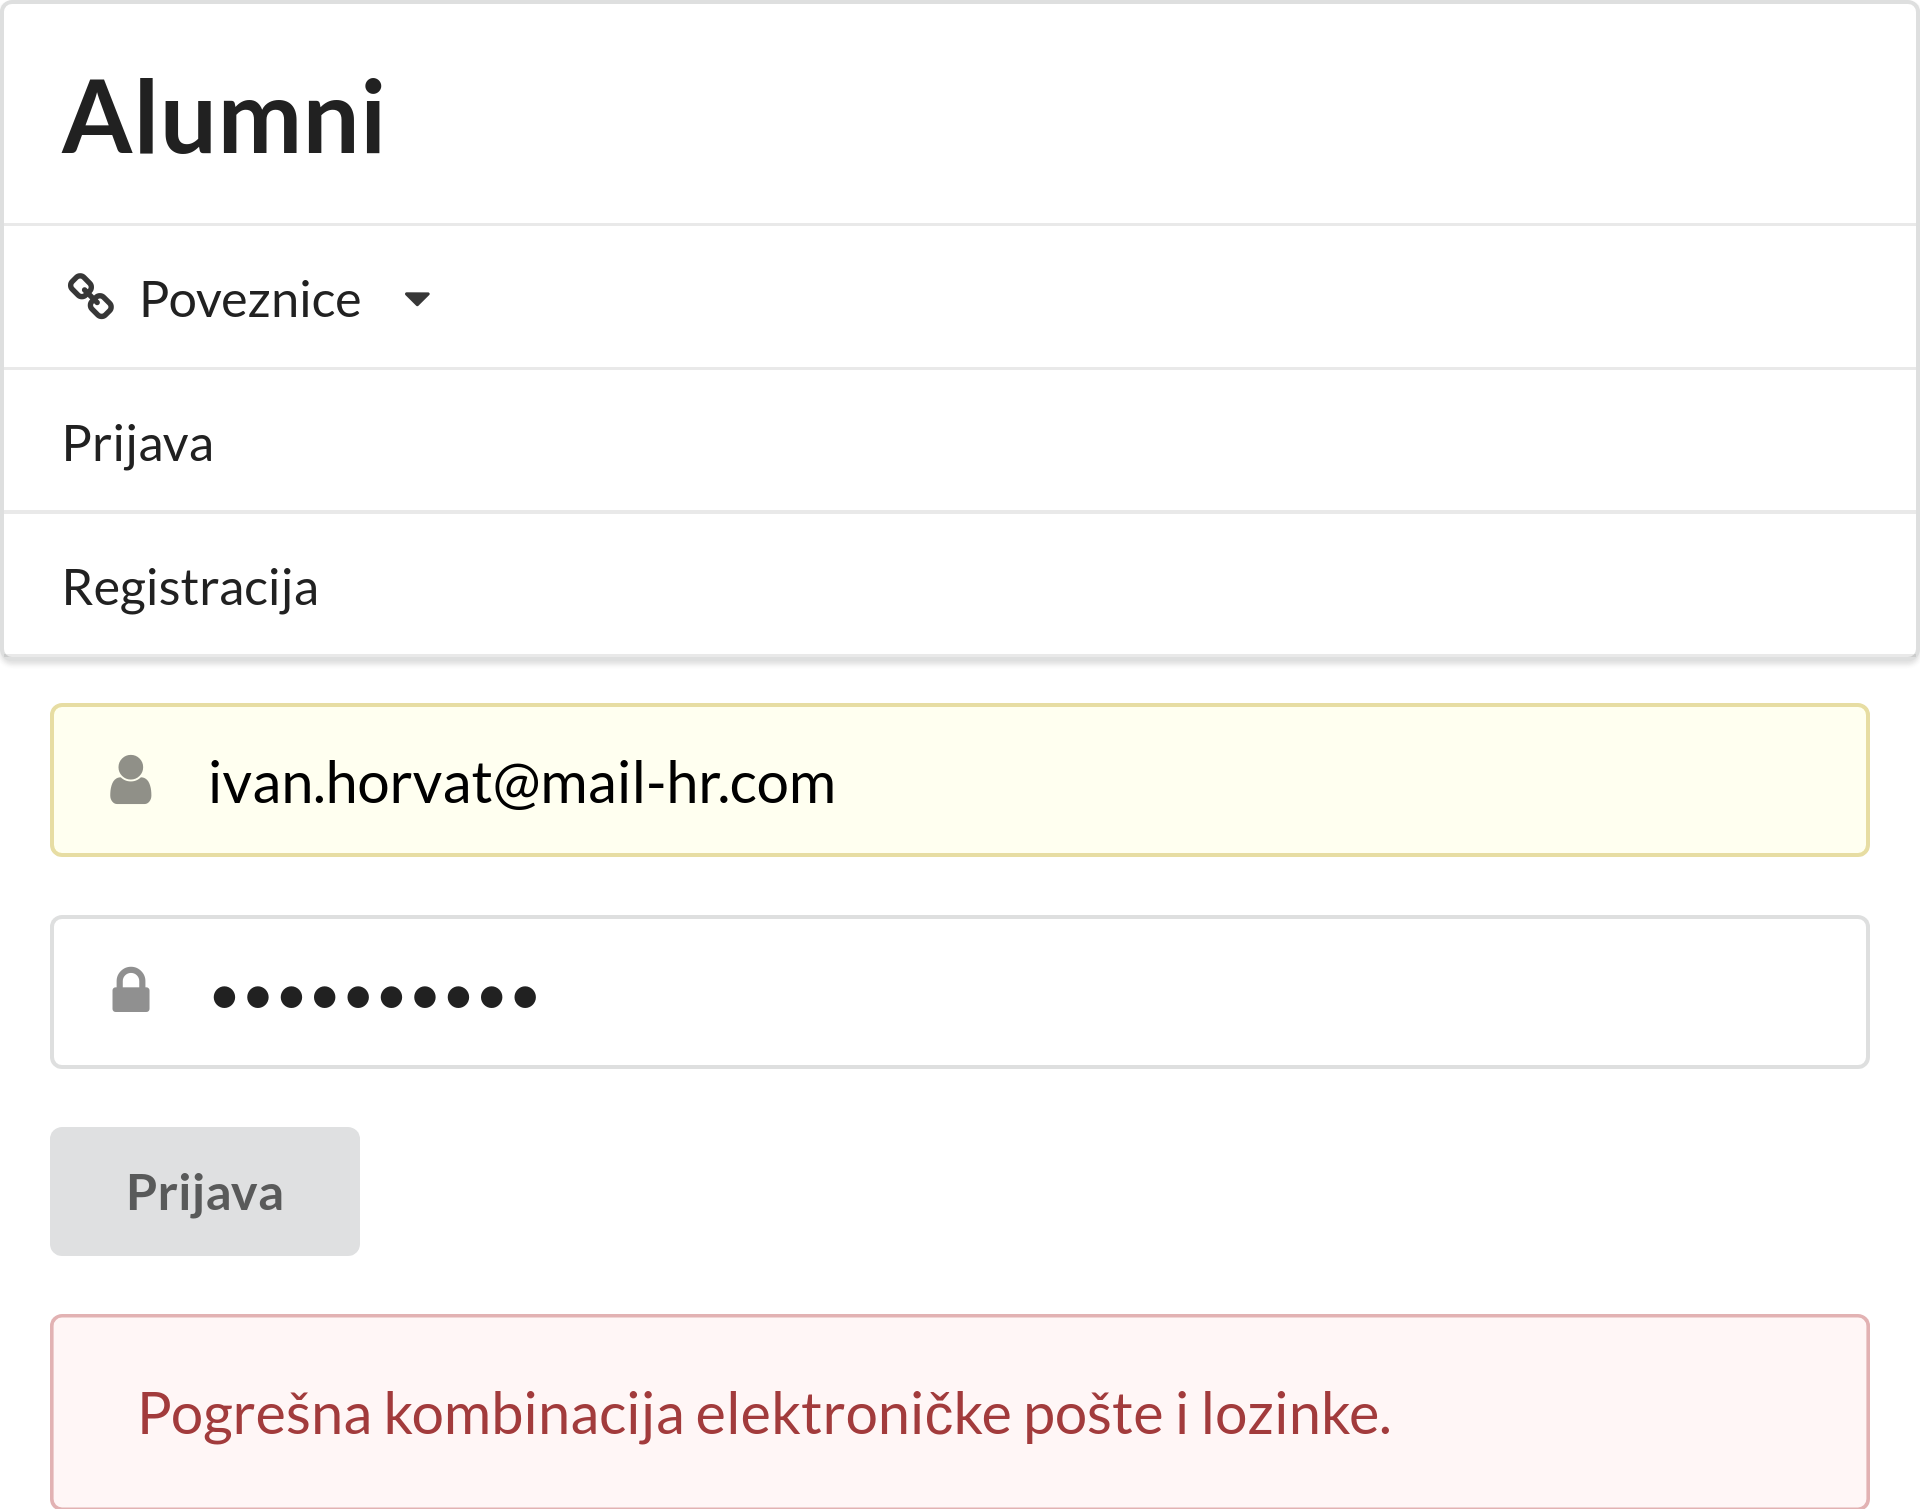
\includegraphics[width=13cm]{slike/prijava.png}
	\caption{Obrazac za prijavu}
	\label{fig:prijava}
\end{figure}

Odabirom "Prijava" na navigacijskoj traci, korisniku se pojavljuje obrazac za prijavu koji se sastoji samo od polja za upis email-a, te polja za upis lozinke. Za oba polja postoji provjera postojanosti, te dodatno za email postoji provjera ispravnosti. Ukoliko se korisnik pokuša prijaviti sa nepostojećim email-om, ili krivo upiše lozinku, prikazati će mu se poruka "Pogrešna kombinacija elektroničke pošte i lozinke". Takva poruka je vrlo popularna u većini aplikacija jer ne otkriva korisniku da li je krivo upisao email ili lozinku, što malo podigne razinu sigurnosti aplikacije.

\subsection{Odjava sa sustava}

\begin{figure}[H]
	\centering
	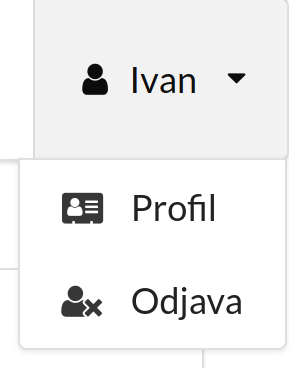
\includegraphics[width=8cm]{slike/odjava.png}
	\caption{Odjava sa sustava}
	\label{fig:odjava}
\end{figure}

Odabirom "Odjava" u padajućem izborniku na desnom kraju trake, korisnik se briše iz trenutne sesije aplikacije i odjavljuje se sa sustava. Time se aplikacija vraća u stanje pregleda koje vidi anoniman korisnik.

\section{Upravljanje korisnicima}
Upravljanje korisnicima je mogućnost koju ima samo administrator, te se sve naredne funkcionalnotsti odnose samo na njega.

\subsection{Pregled svih korisnika}

\begin{figure}[H]
	\centering
	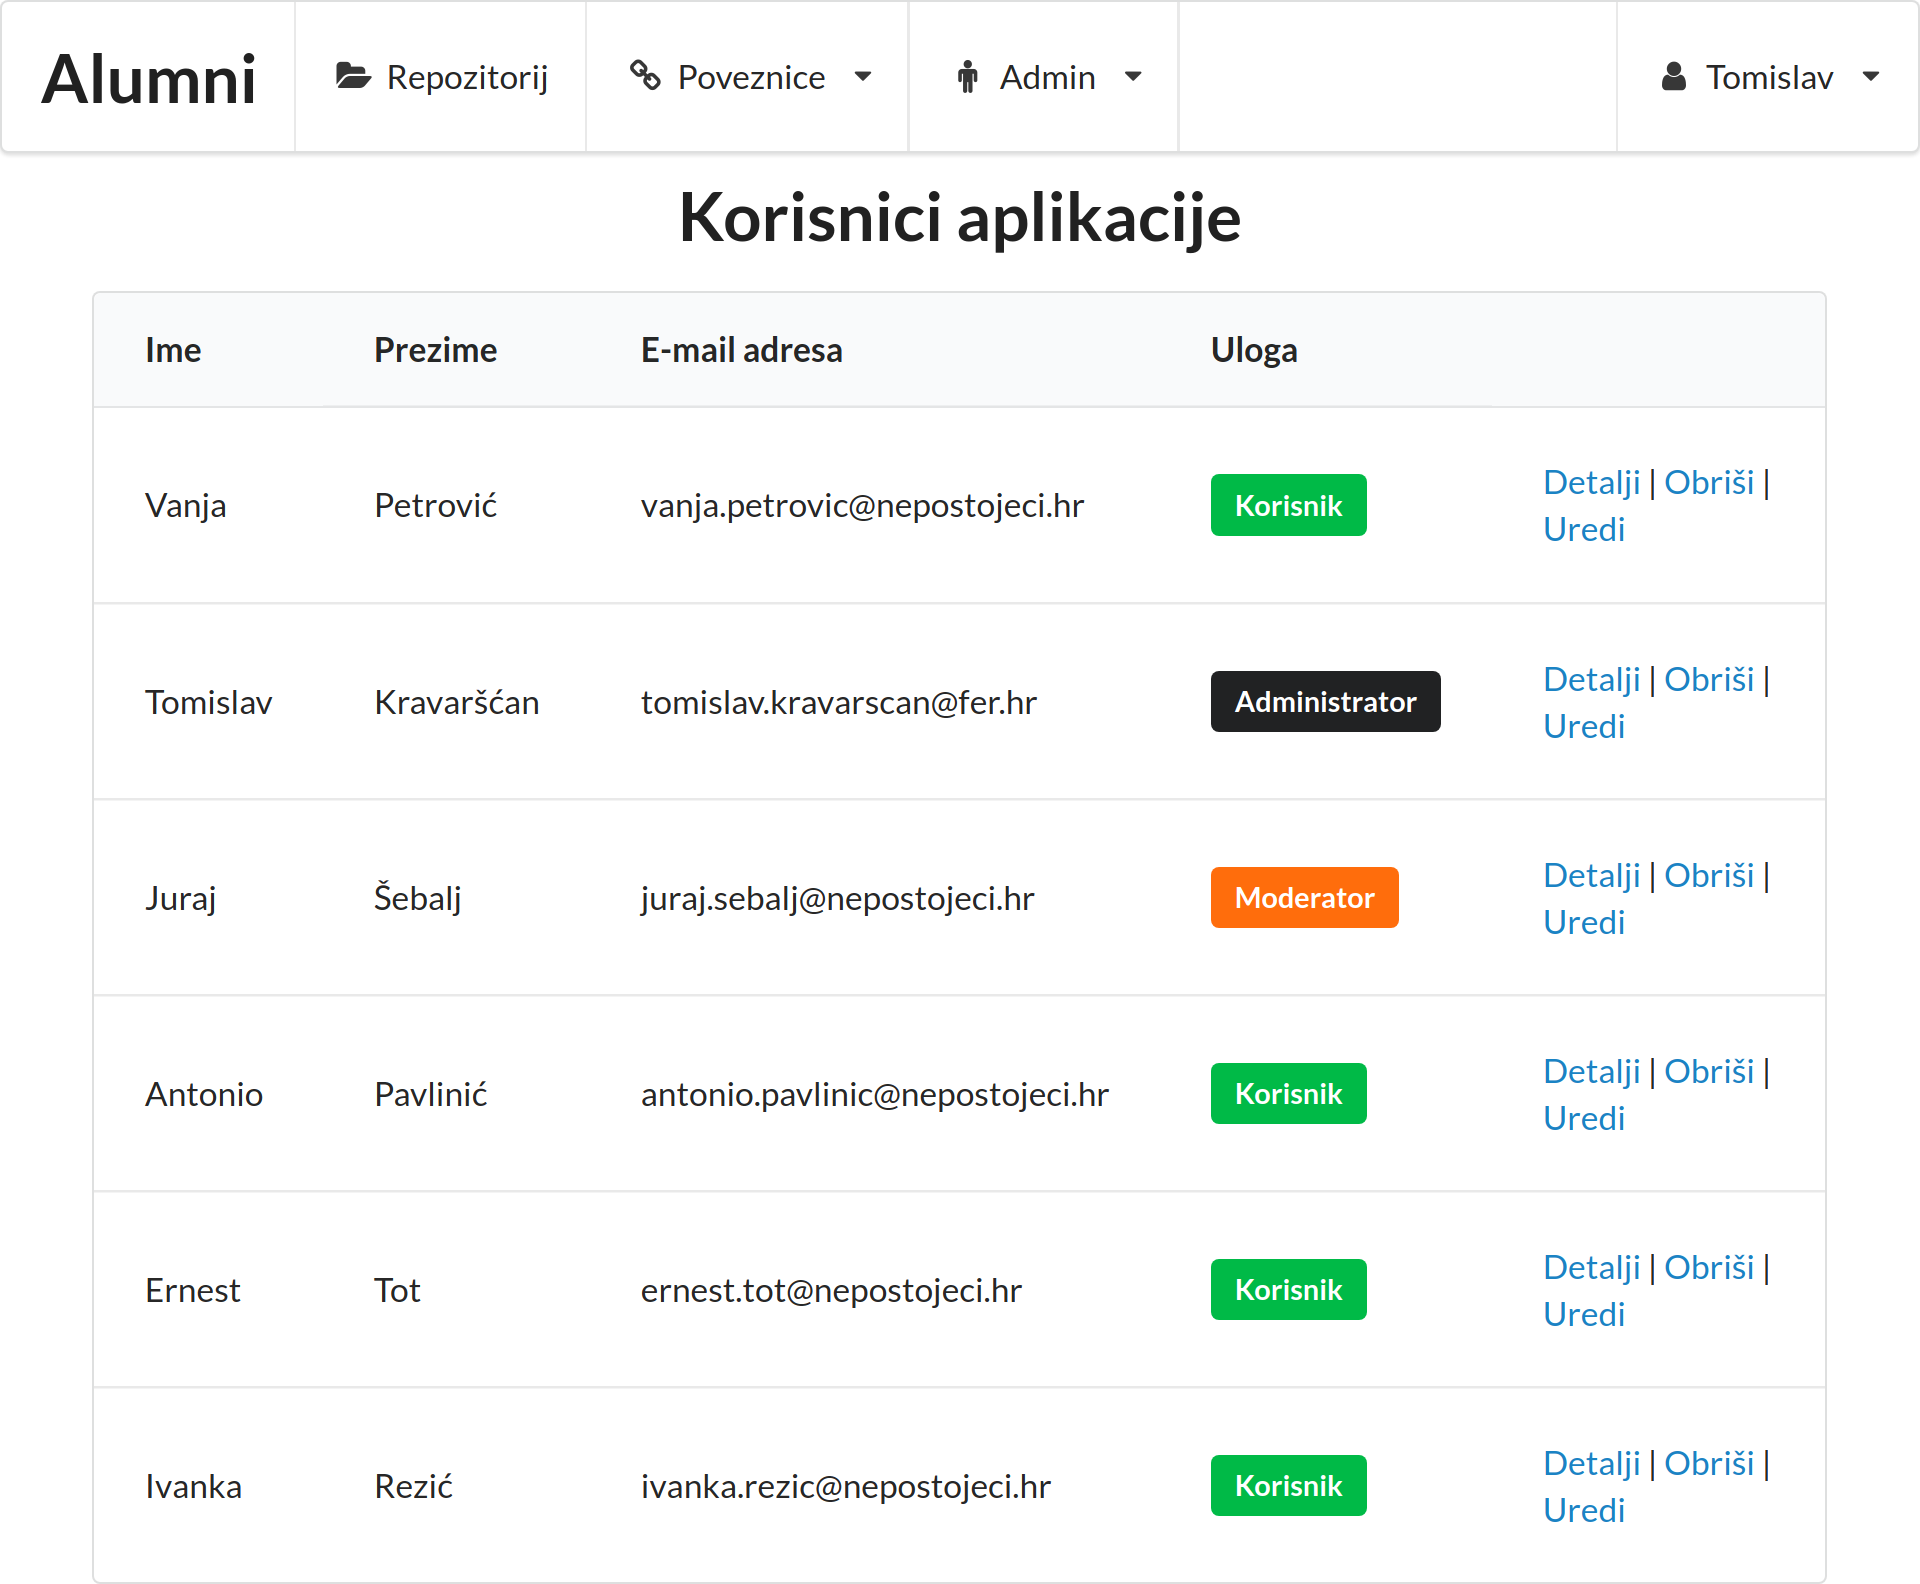
\includegraphics[width=13cm]{slike/korisnici.png}
	\caption{Pregled svih korisnika}
	\label{fig:korisnici}
\end{figure}

Pregled svih korisnika koji se nalaze u aplikaciji ostvaruje se odabirom "Korisnici" u padajućem izborniku "Admin" na navigacijskoj traci. Na tom pregledu su vidljive samo osnovne informacije o korisniku kao što su ime, prezime, email, te uloga korisnika. Osim toga, na desnoj strani zapisa svakog korisnika je moguće odabrati prikaz detalja korisnika, brisanje korisnika te uređivanje korisničkih podataka.

\subsection{Pregled korisničkog računa}

\begin{figure}[H]
	\centering
	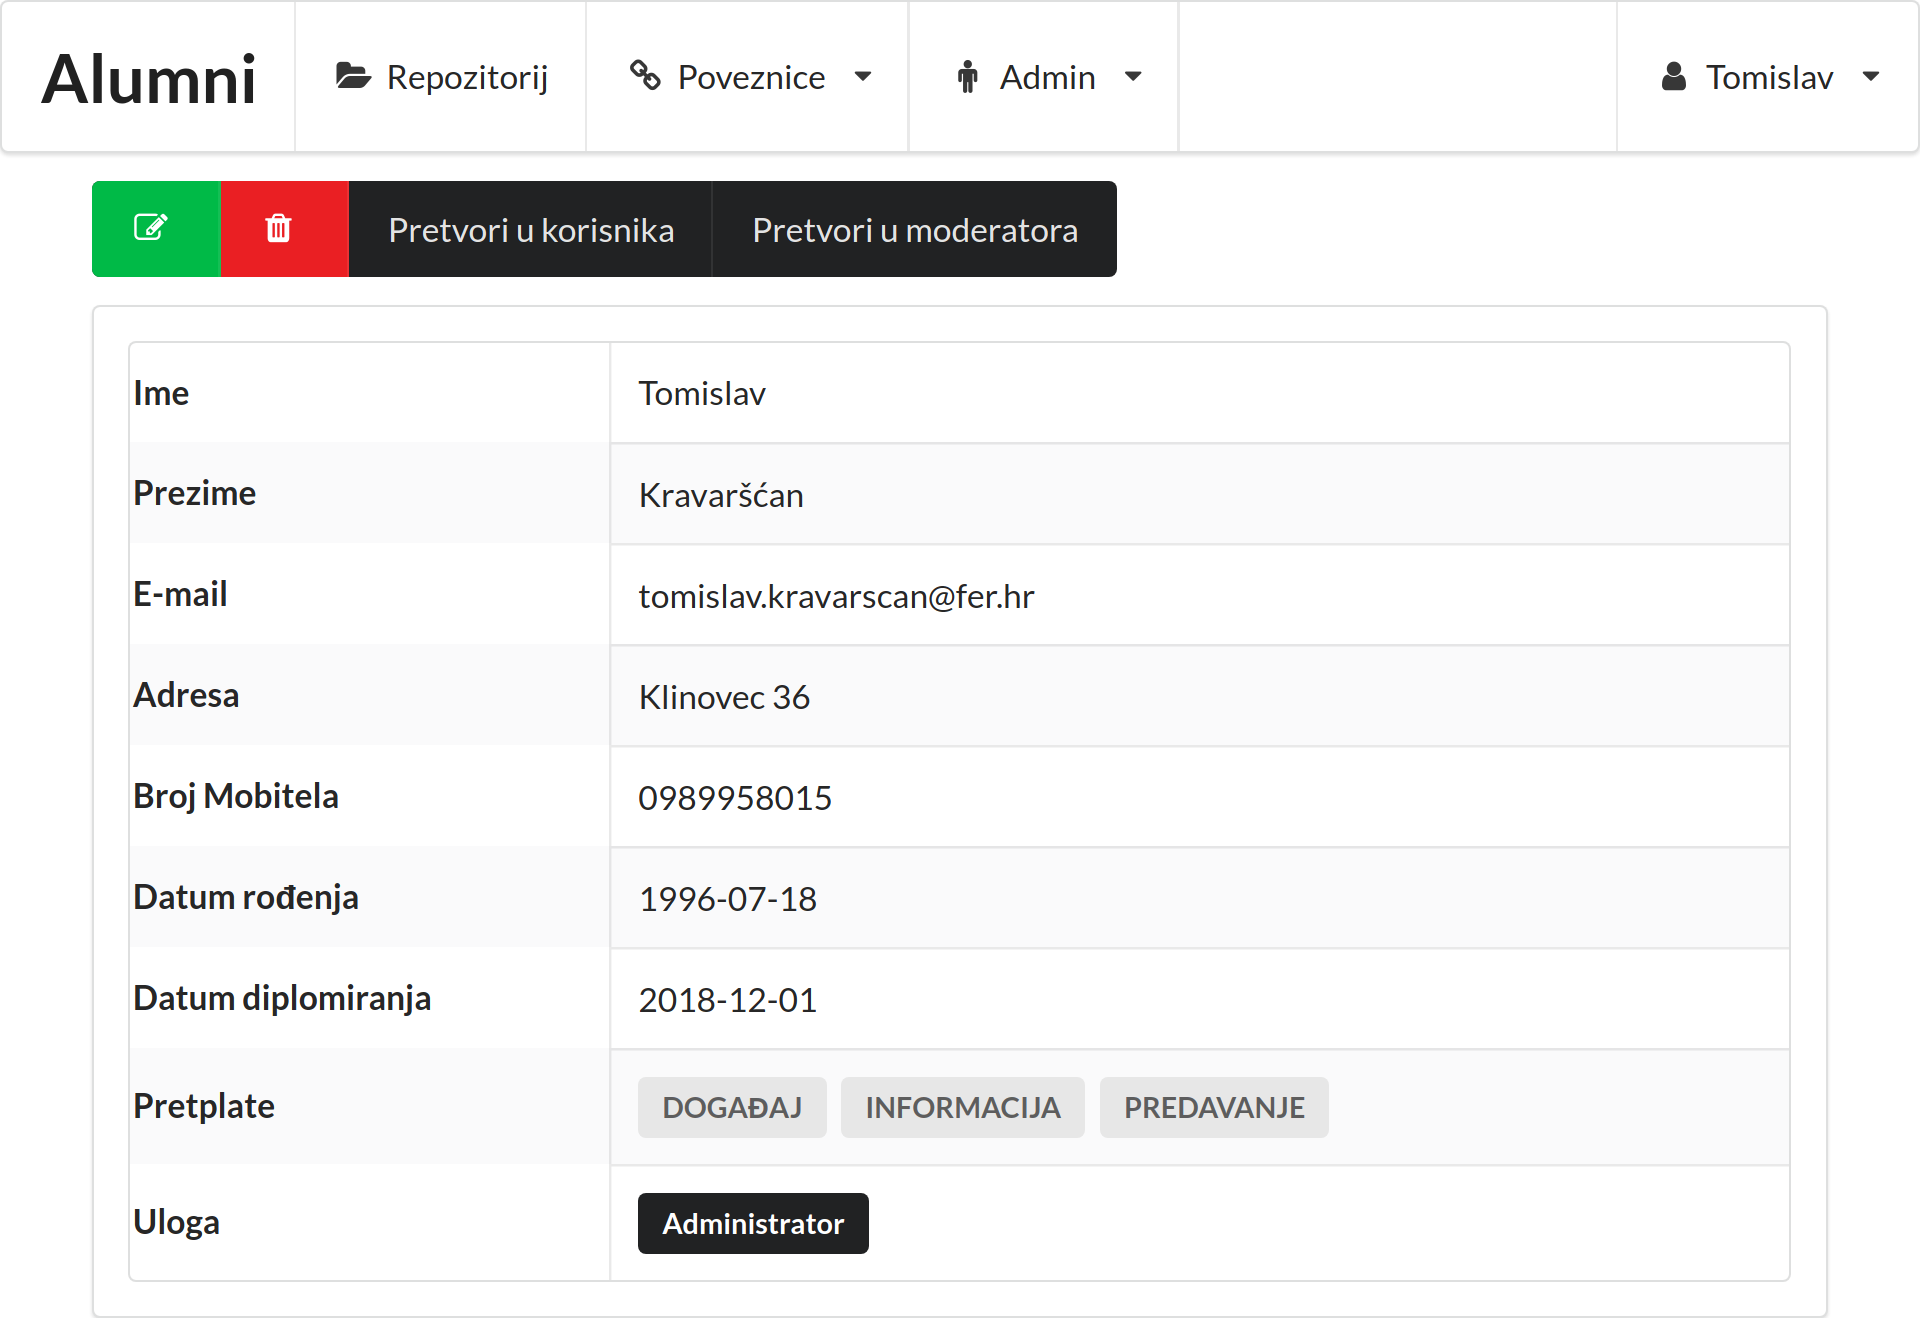
\includegraphics[width=13cm]{slike/profil.png}
	\caption{Korisnički profil}
	\label{fig:profil}
\end{figure}

Administrator može vidjeti sve korisničke račune u sustavu, pa do pregleda korisničkog računa može doći na dva načina: putem padajućeg izbornika u navigacijskoj traci, gdje odabire pregled vlastitog korisničkog računa, te odabirom poveznice detalji na pregledu svih korisnika.

Na pregledu korisničkog računa, imamo sve bitne informacije o korisniku kao što su ime, prezime, email, adresa, broj mobitela, datum rođenja, datum diplomiranja te uloga. Običan korisnik pregledom svog računa može odabrati opciju uređivanja i brisanja pri vrhu stranice za pregled računa, dok administrator ima još opcije promijene uloge korisnika.

\subsection{Uređivanje korisničkog računa}

\begin{figure}[H]
	\centering
	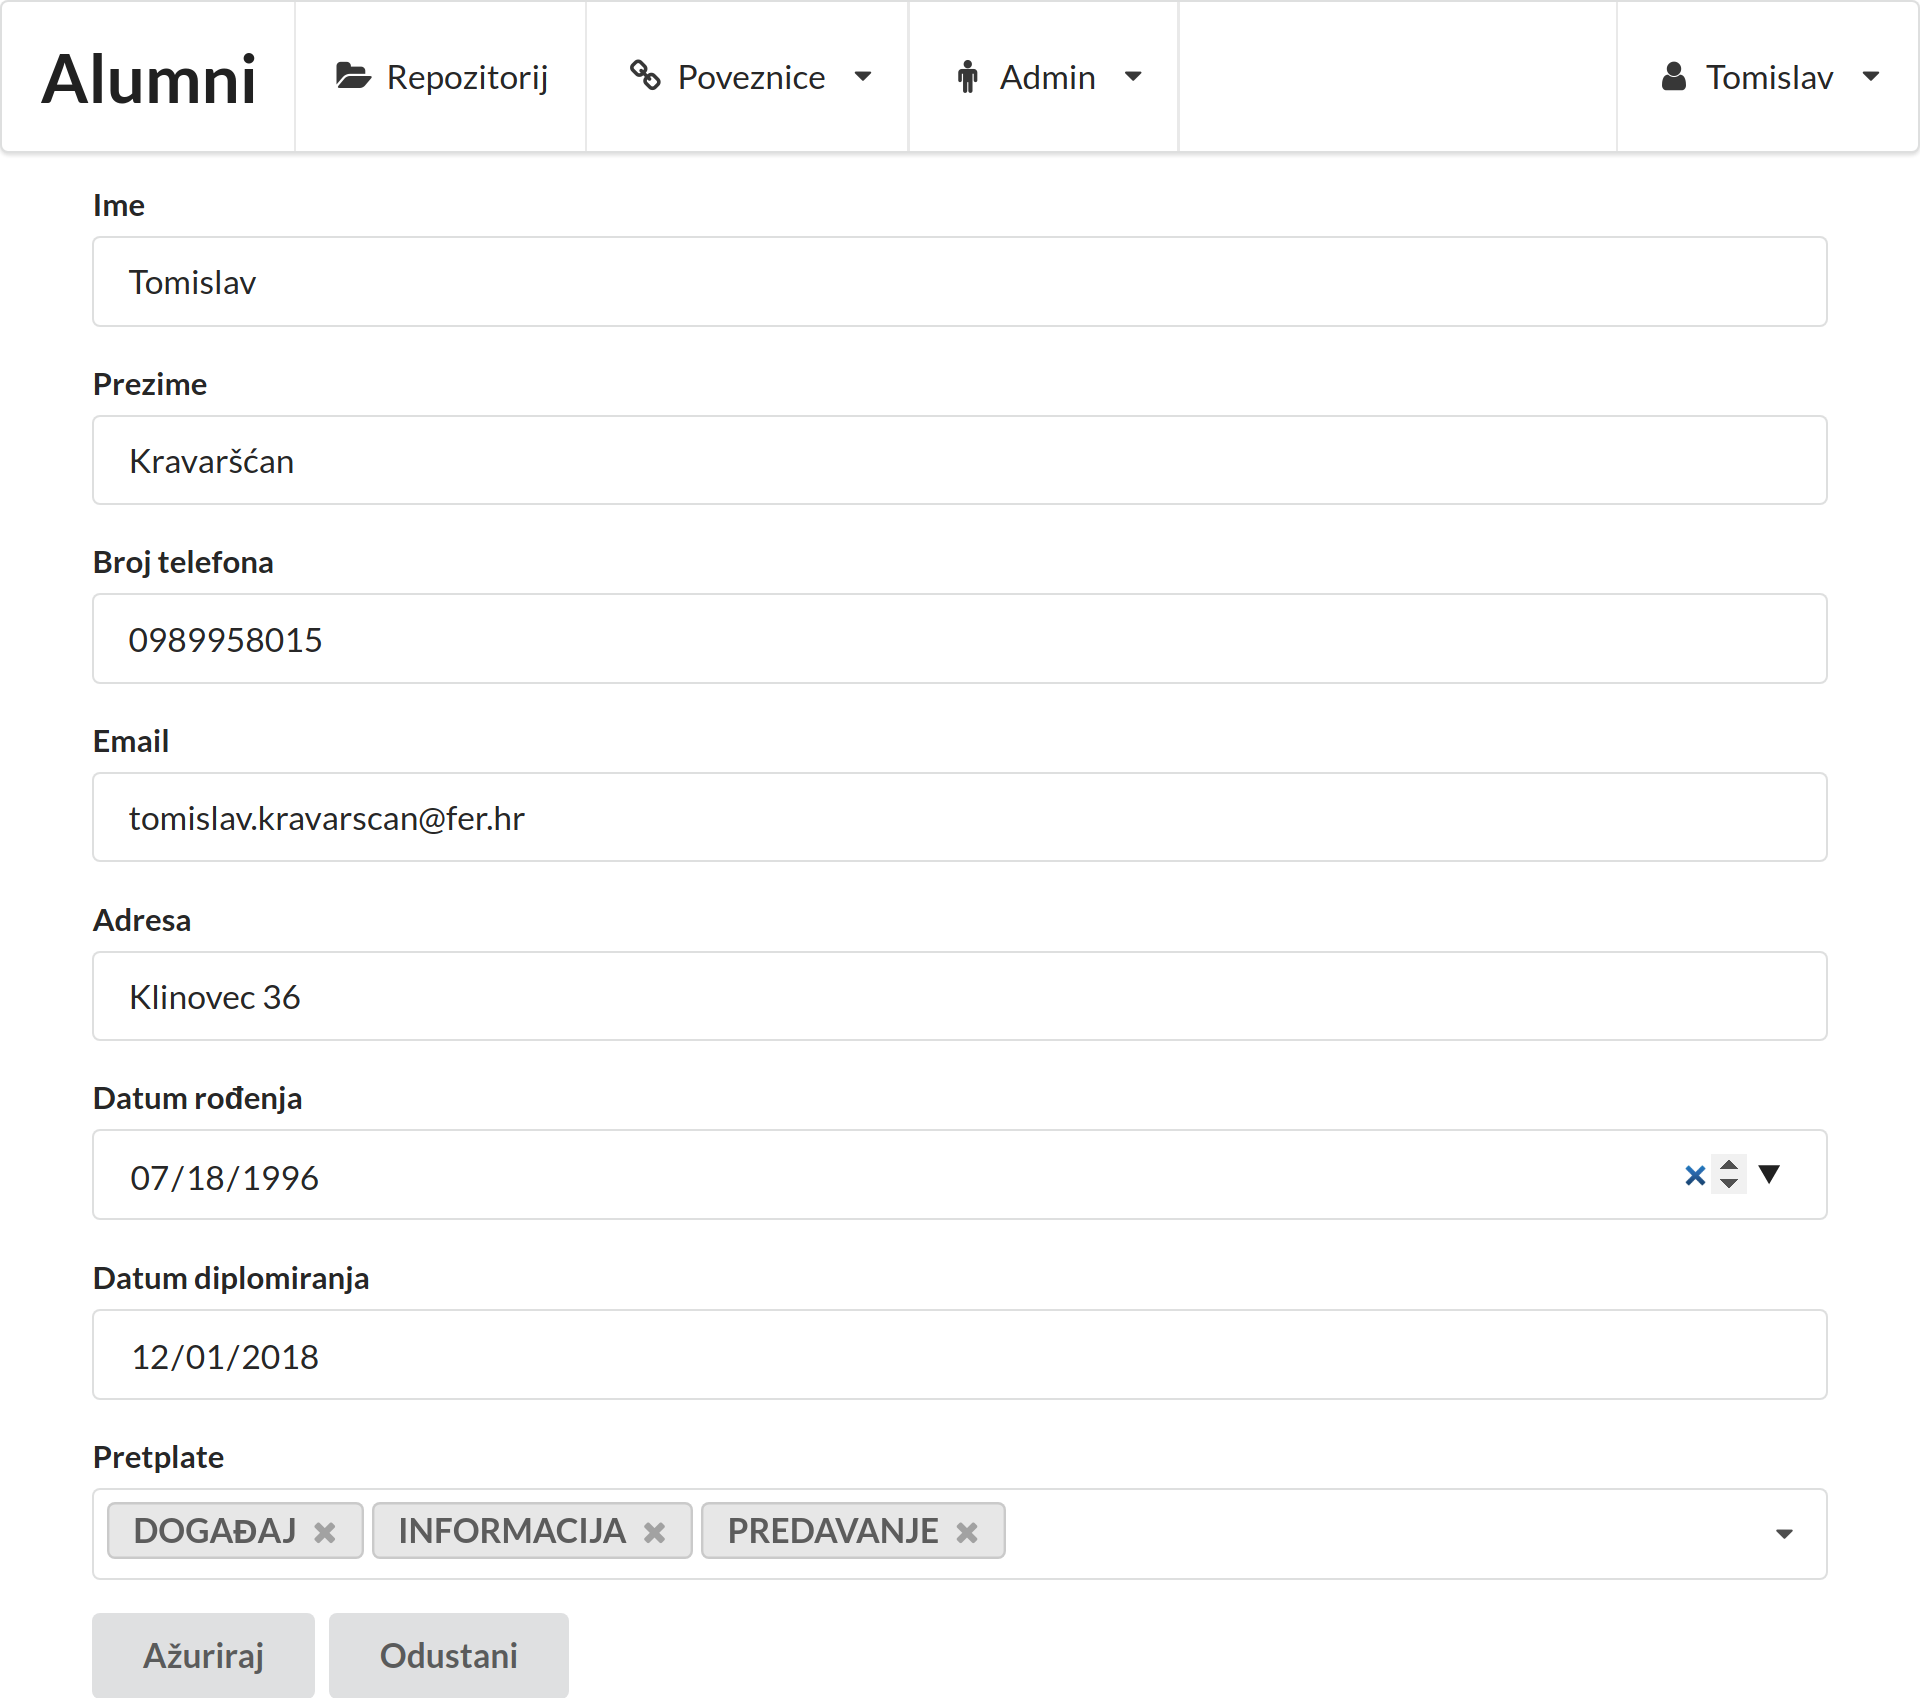
\includegraphics[width=13cm]{slike/uredi-profil.png}
	\caption{Obrazac za uređivanje profila}
	\label{fig:uredi-profil}
\end{figure}

Stranica za uređivanje korisničkog računa je vrlo slična stranici za registraciju, osim što nema upisa lozinke. Korisniku se pojavljuje obrazac gdje su sva polja već ispunjena njegovim podacima. Promijenom bilo kojeg podatka korisnički se račun ažurira i to je odmah vidljivo. Dodatna mogućnost kod uređivanja korisničkog računa je dodavanje pretplata na kategorije postova, o tome će biti više u poglavlju "Sustav pretplata".

\subsection{Promijena uloge korisnika}
Na pregledu korisničkog profila, administrator može promijeniti ulogu korisnika odnosno pretvaranje korisnika u one uloge koje postoje u sustavu, a da ih korisnik trenutno nema. Promijenom uloge korisnik preuzima sve mogućnosti te uloge u sustavu.

\subsection{Brisanje korisničkog računa}
Brisanjem korisničkog računa se iz baze podataka obrišu svi podaci korisnika, te se brišu svi njegovi komentari na postove.

\section{Upravljanje poveznicama}
Poveznice su vrlo bitne za upravljanje bilo kojom udrugom, pa je sustavom za upravljanje poveznicama administratoru koji nije upoznat sa html sintaksom i nije u mogućnosti ugraditi poveznice izravno u kod stranice, administratoru omogićeno lagano dodavanje poveznica.

\subsection{Pregled svih poveznica}

\begin{figure}[H]
	\centering
	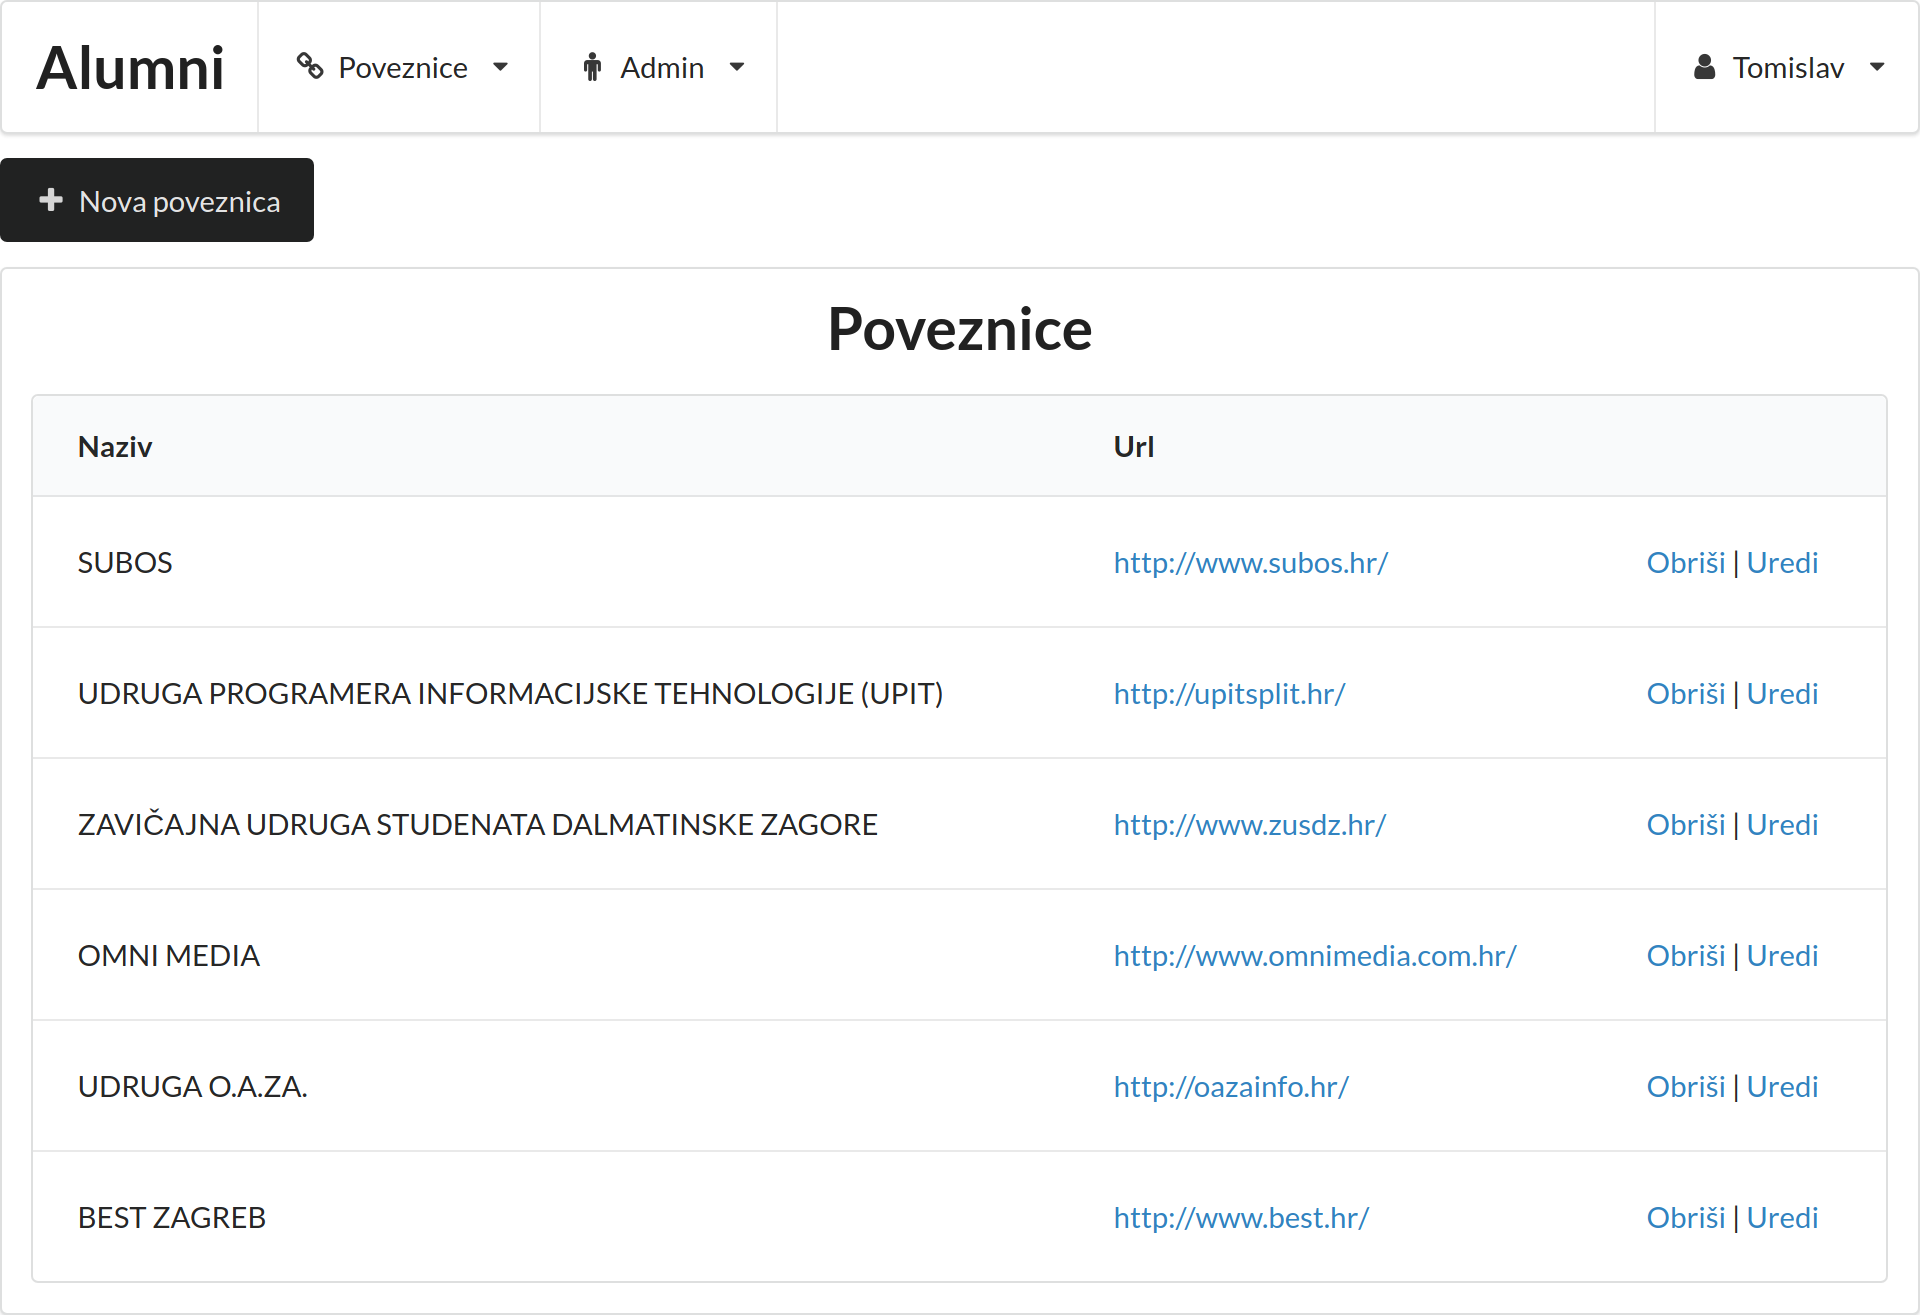
\includegraphics[width=13cm]{slike/poveznice.png}
	\caption{Pregled svih poveznica}
	\label{fig:poveznice}
\end{figure}

Osim što se sve poveznice mogu vidjeti u padajućem izborniku navigacijske trake, za administratora je bitno da ima popis svih poveznica uz dodatne opcije uređivanja i brisanja svake poveznice, slično kao i kod pregleda svih korisnika. Do tog pregleda poveznica dolazi se putem padajućeg izbornika "Admin", odabirom "Stranica poveznica".

\subsection{Dodavanje nove poveznice}

\begin{figure}[H]
	\centering
	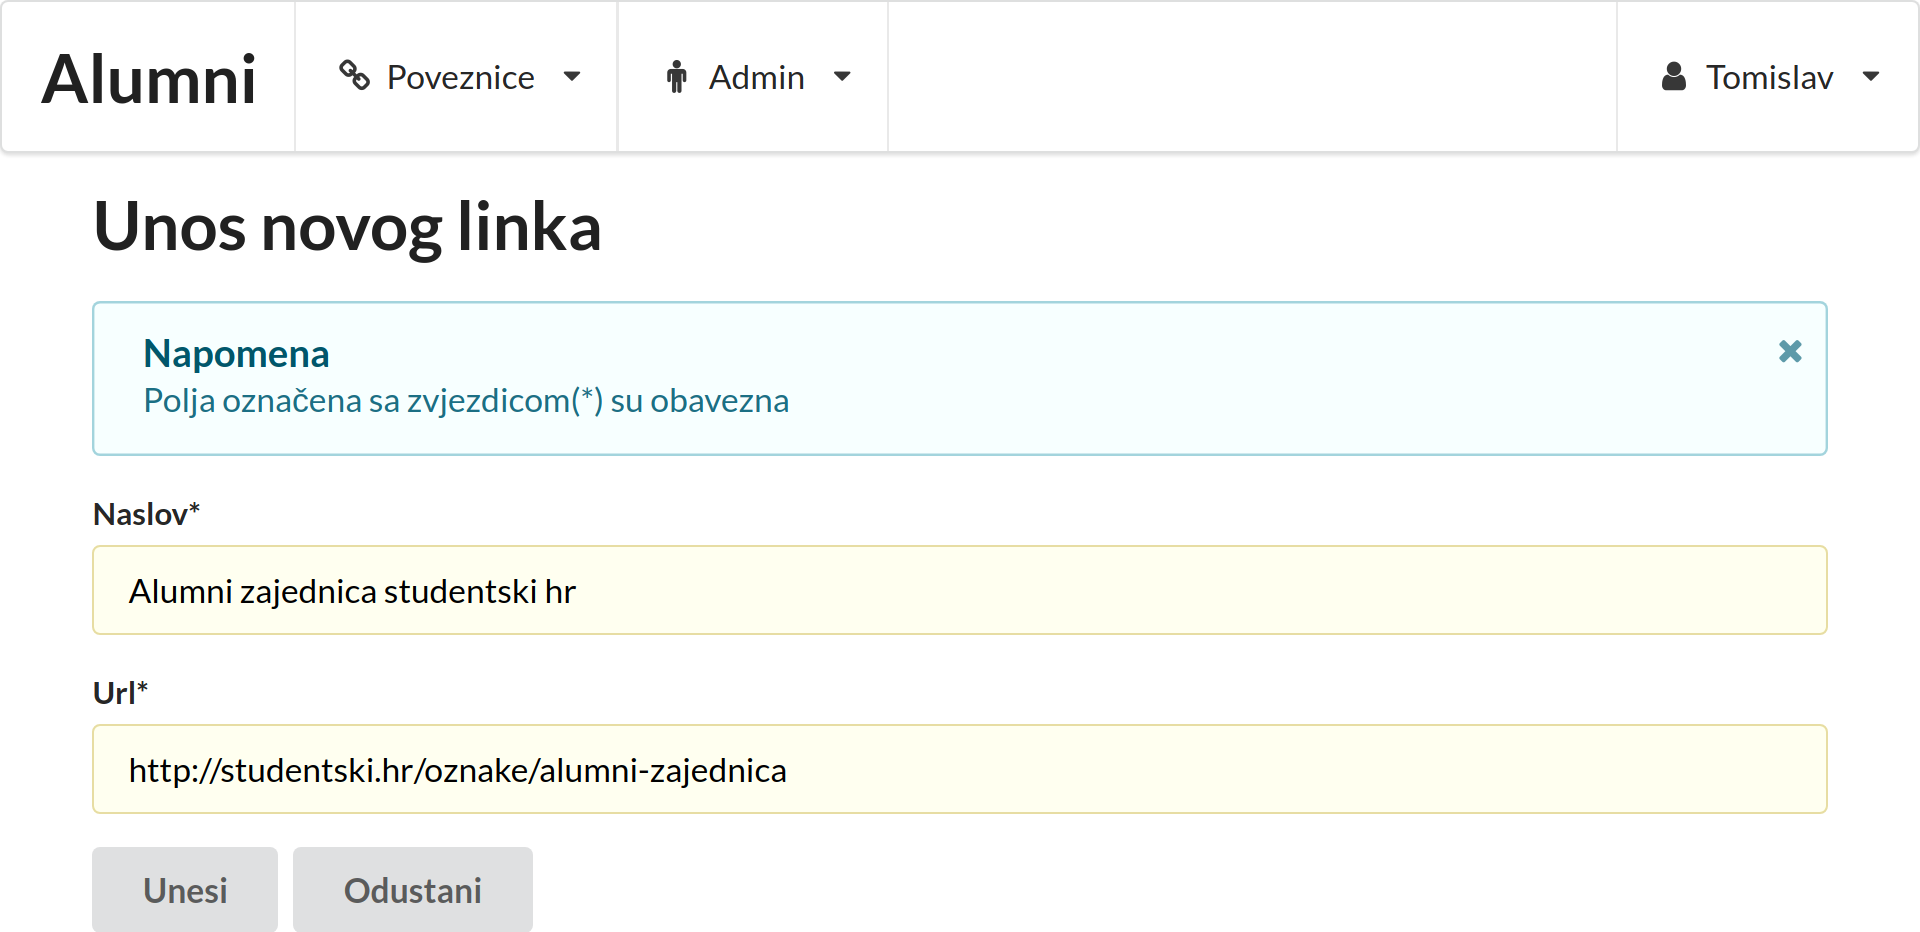
\includegraphics[width=13cm]{slike/nova-poveznica.png}
	\caption{Obrazac za novu poveznicu}
	\label{fig:nova-poveznica}
\end{figure}

Odabirom opcije dodavanja nove poveznice na vrhu pregleda svih poveznica, korisniku se pojavljuje jednostavan obrazac koji ima samo polja naslov i url. Oba polja su obavezna i ne upisivanje bilo kojeg rezultira pogreškom, dodatno, url mora biti ispravnog formata i započinjati sa oznakom protokola.

\subsection{Uređivanje poveznice}
Odabirom opcije uređivanja poveznice na desnoj strani zapisa svake poveznice prikazuje se isti obrazac kao i kod stvaranja poveznice, uz to da su podaci o poveznici već upisani. 

\subsection{Brisanje poveznice}
Odabirom brisanja poveznice, poveznica se uklanja iz sustava.

\section{Upravljanje kategorijama}
Svaki post u sustavu mora imati određenu kategoriju. Zbog olakšanog proširivanja funkcionalnosti aplikacije administratoru je omogućeno dinamičko stvaranje novih kategorija postova. 

\subsection{Pregled svih kategorija}

\begin{figure}[H]
	\centering
	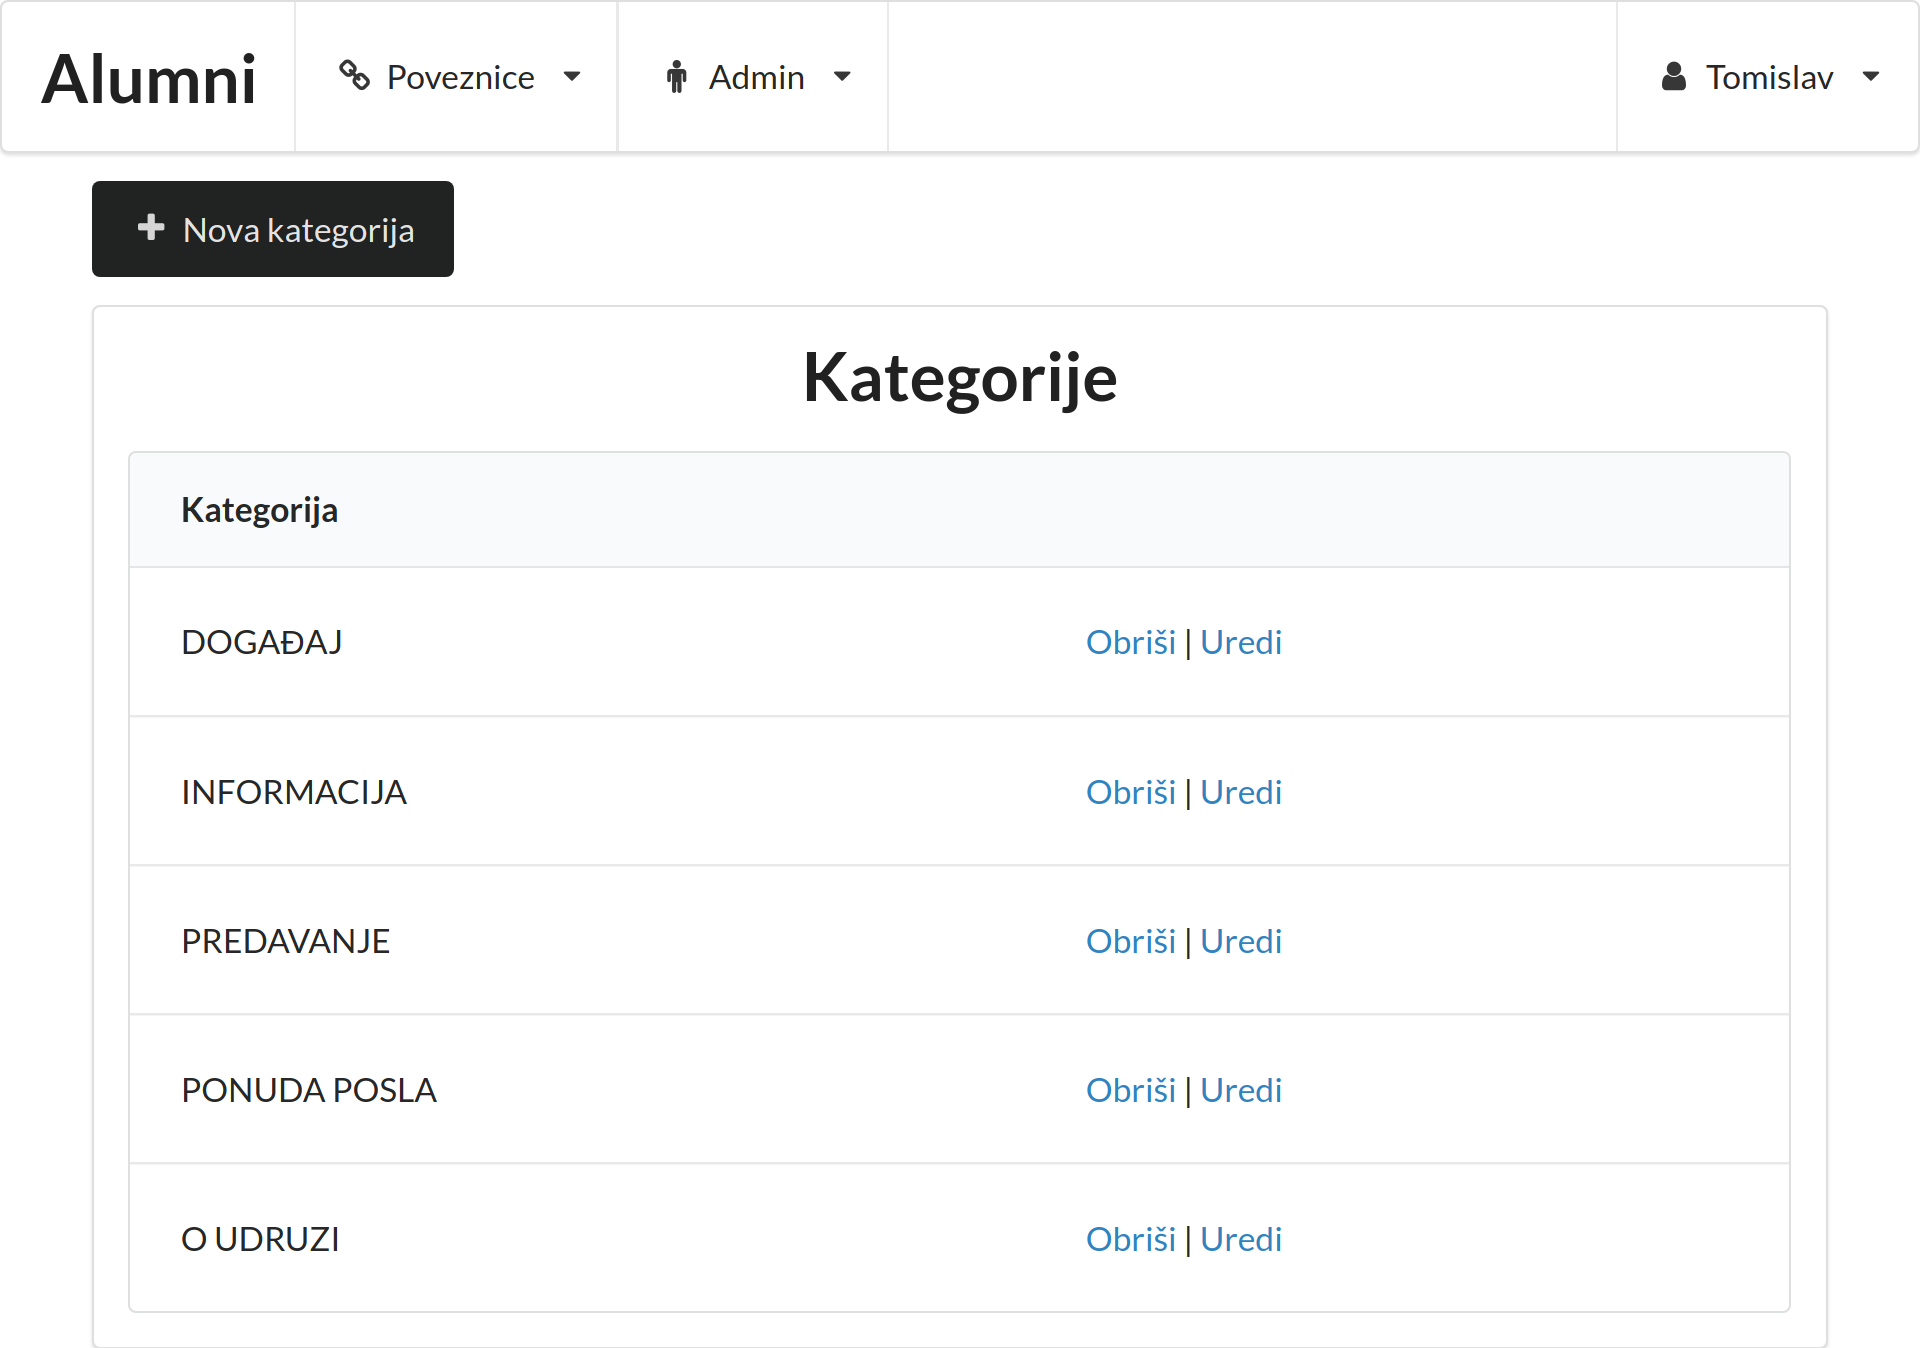
\includegraphics[width=13cm]{slike/kategorije.png}
	\caption{Pregled svih kategorija}
	\label{fig:kategorije}
\end{figure}

Do pregleda svih kategorija dolazi se putem padajućeg izbornika "Admin" u navigacijskoj traci, odabirom na "Kategorije". Za svaku kategoriju prikazan je samo njen naziv, te postoje mogućnosti brisanja i uređivanja. Osim toga, na vrhu stranice je opcija dodavanja nove kategorije.

\subsection{Dodavanje nove kategorije}

\begin{figure}[H]
	\centering
	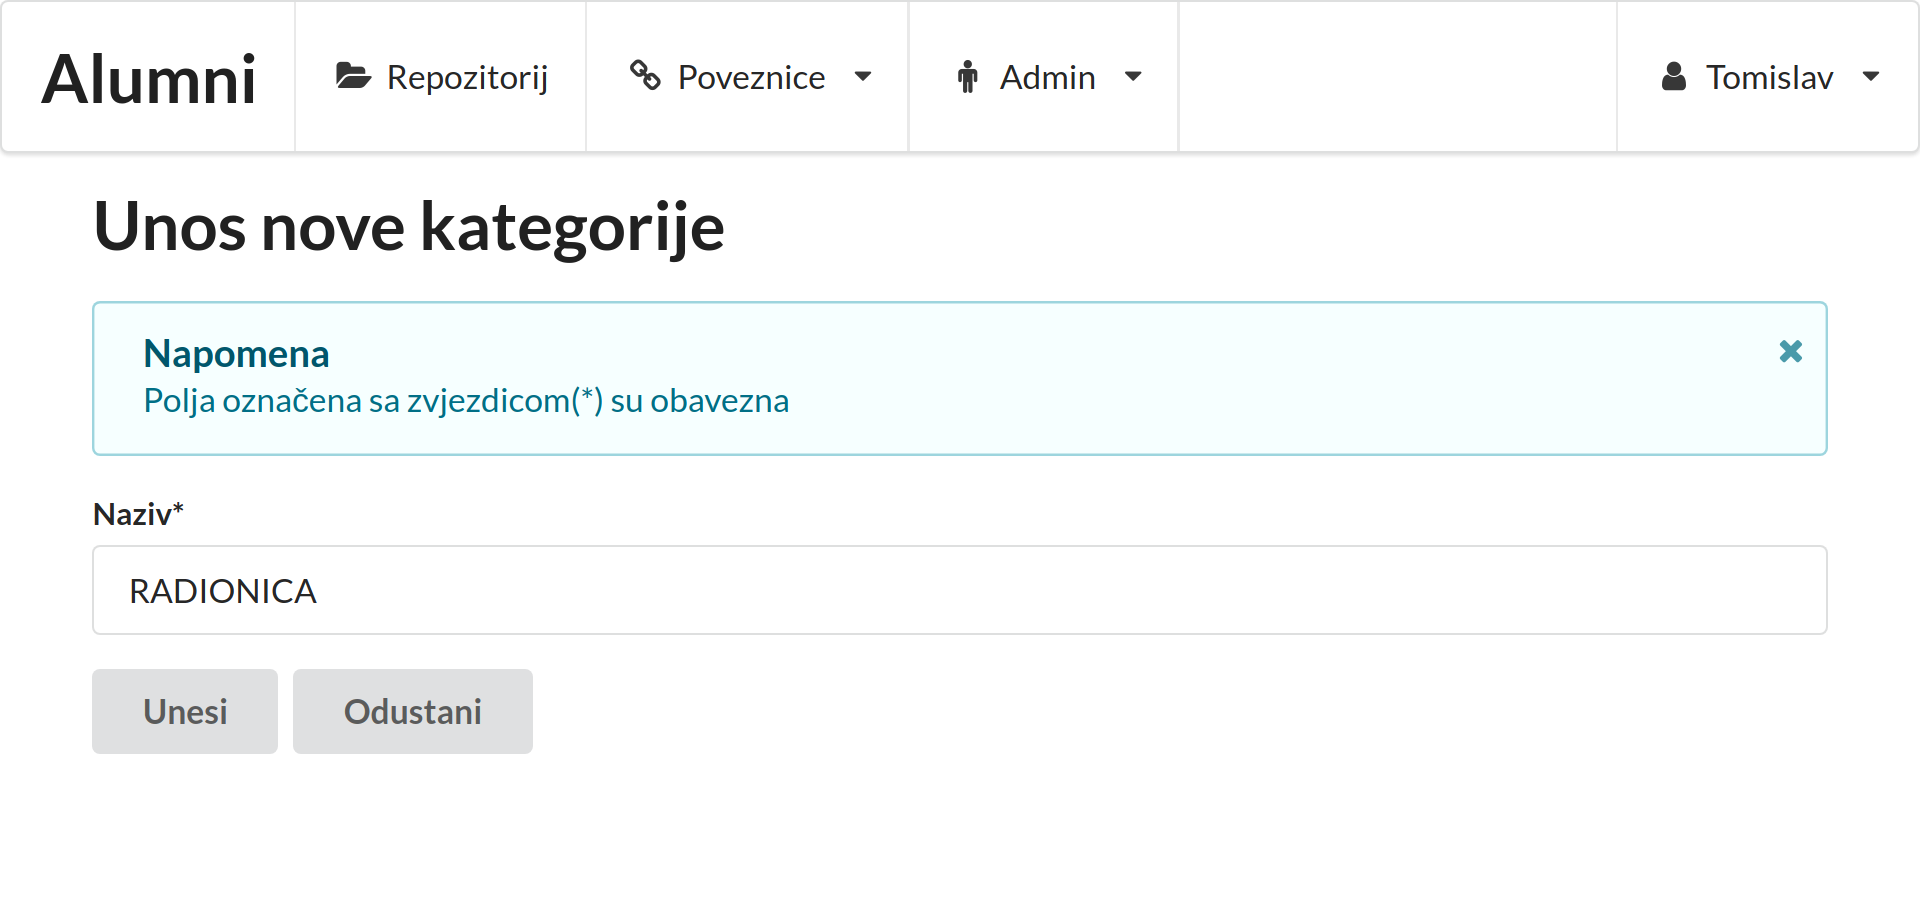
\includegraphics[width=13cm]{slike/nova-kategorija.png}
	\caption{Obrazac za novu kategoriju}
	\label{fig:nova-kategorija}
\end{figure}

Dodavanje nove kategorije je vrlo jednostavno i obrazac ima samo jedno polje, naslov kategorije. To polje naravno ne smije biti prazno.

\subsection{Uređivanje kategorije}
Kategorija se može urediti, i to se obavlja na isti način kao i kod stvaranja.

\subsection{Brisanje kategorije}
Kod pokušaja brisanja kategorije, ako postoje postovi koji su te kategorije, aplikacija će nam zabraniti taj pokušaj. Prvo je potrebno obrisati sve postove s tom kategorijom, ili svim takvim postovima ukloniti kategoriju koju želimo obrisati.

\section{Upravljanje postovima}
Upravljane postovima je gotovo najbitnija funkcionalnost kod programske podrške za neku zajednicu. Vrlo je bitno na pregledan način korisnicima prikazati sve relevantne novosti.

\subsection{Pregled svih postova}

\begin{figure}[H]
	\centering
	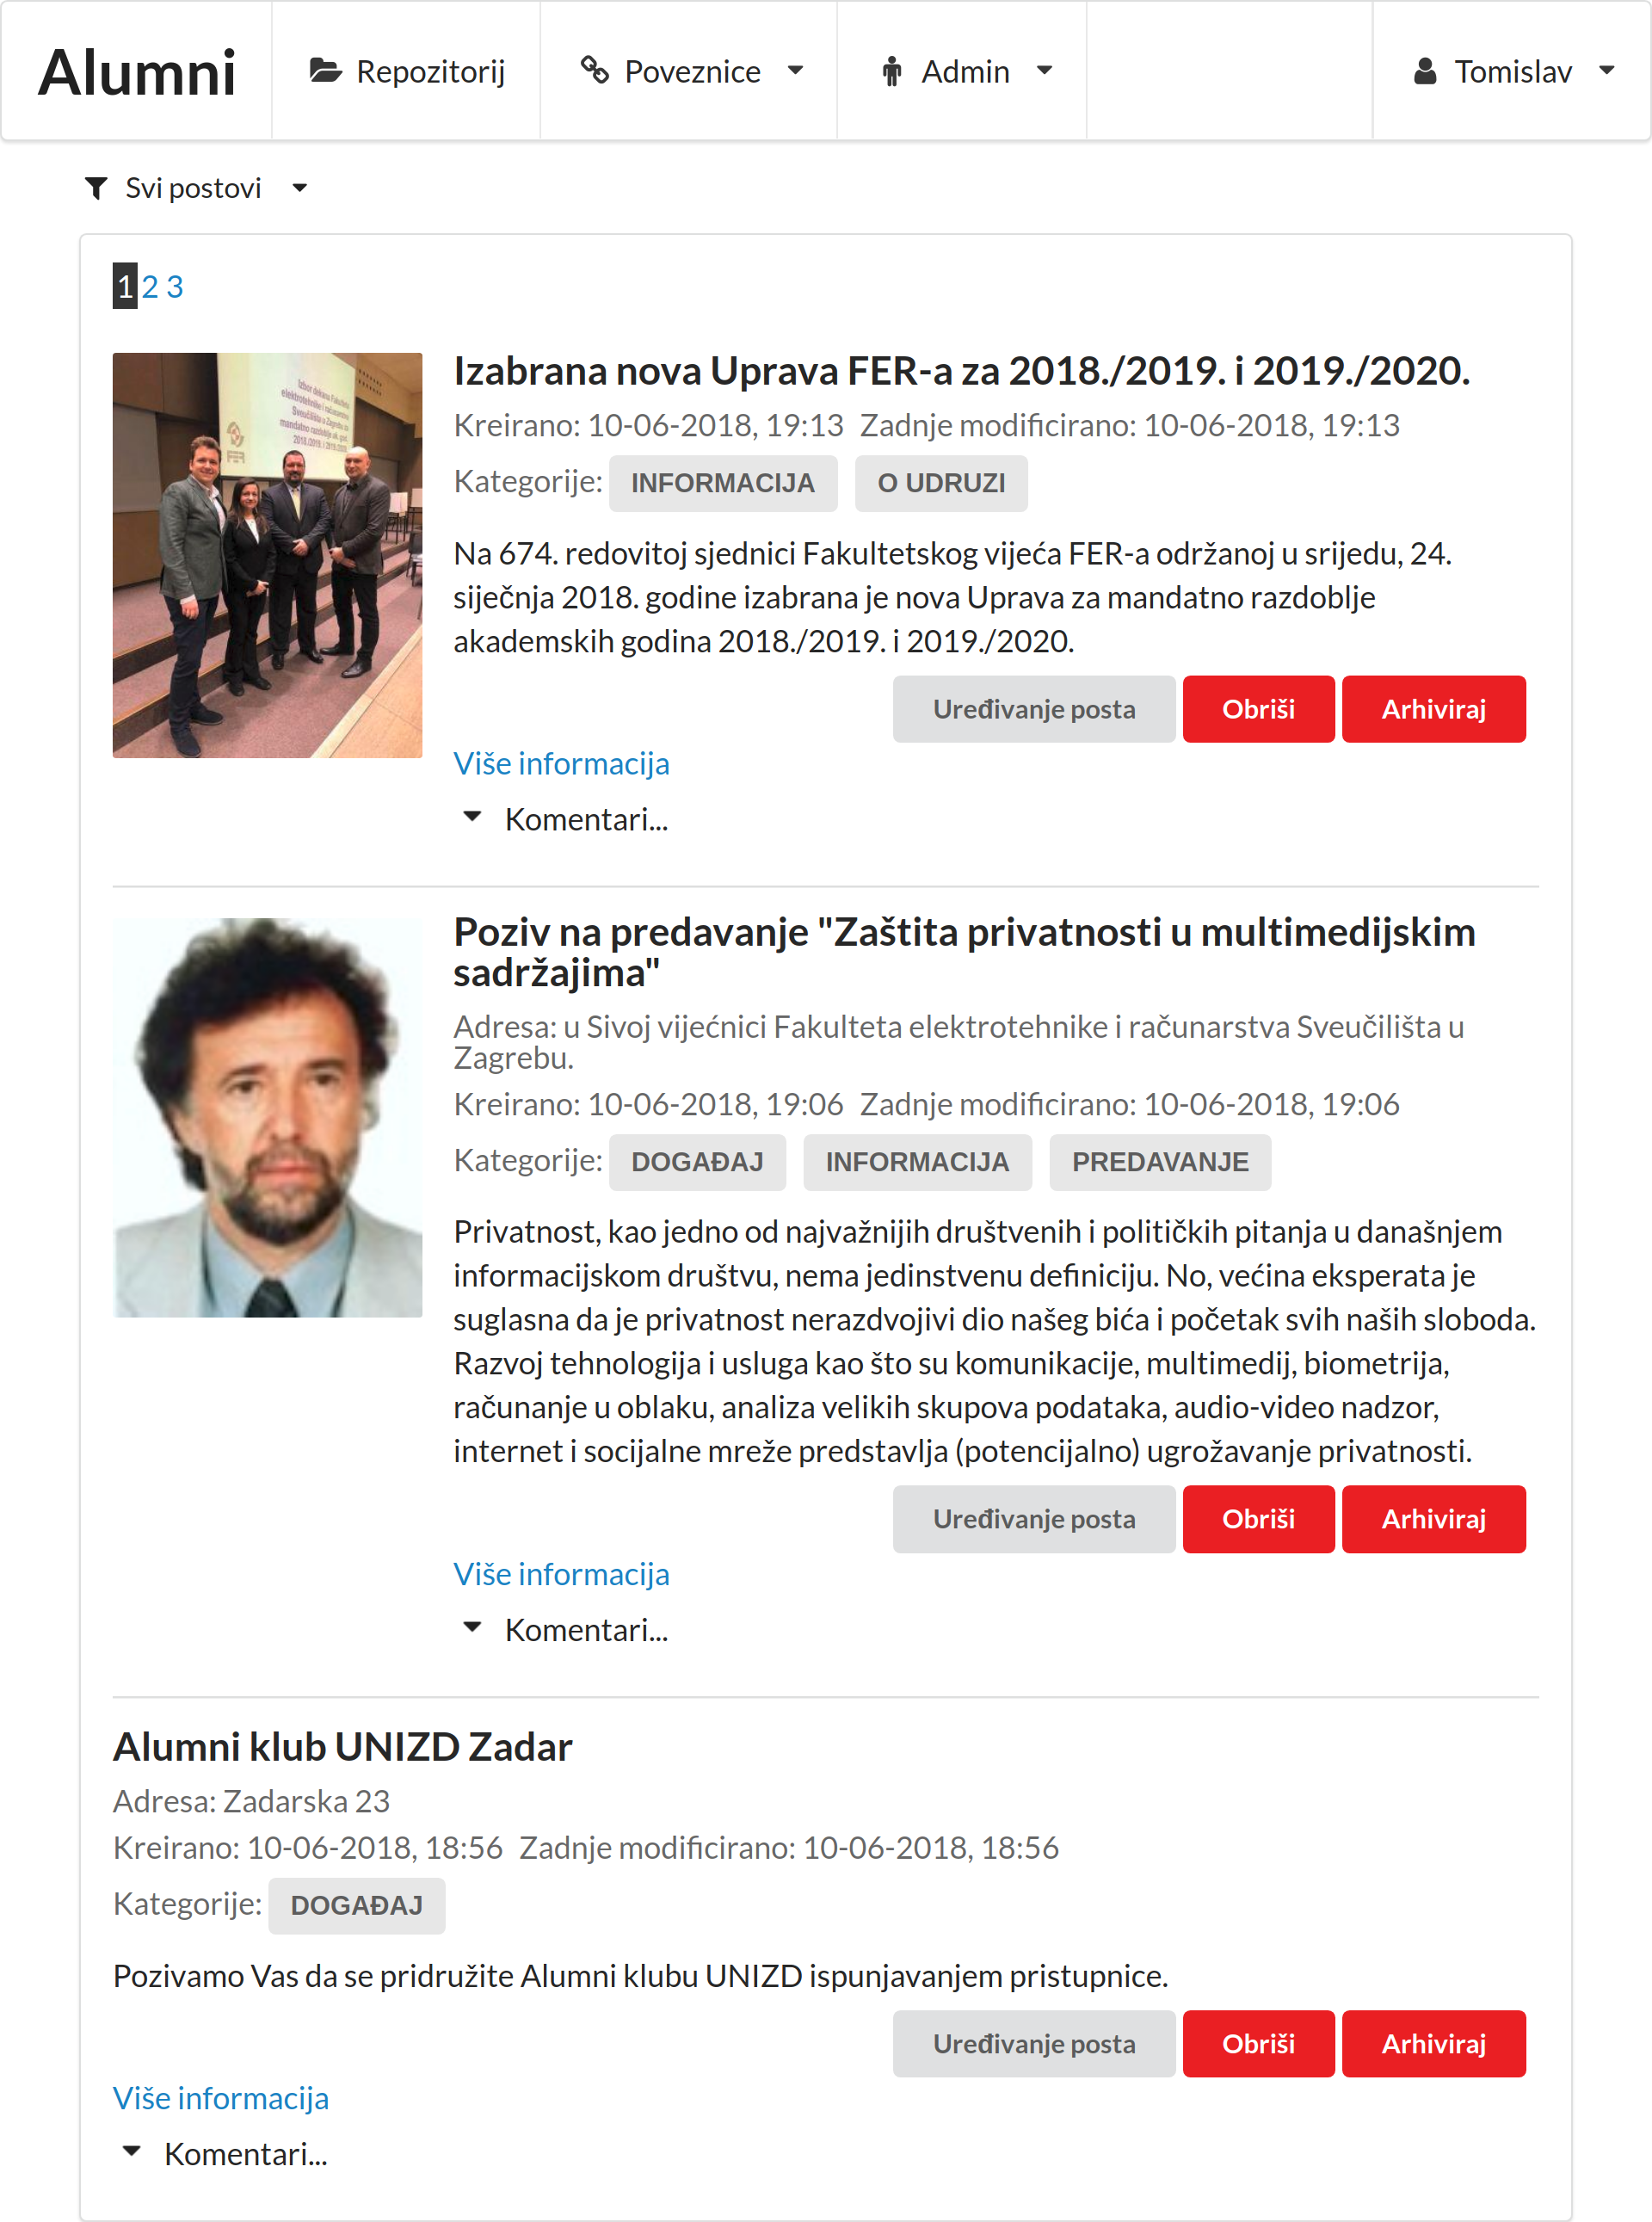
\includegraphics[width=13cm]{slike/postovi.png}
	\caption{Početna stranica - pregled svih postova}
	\label{fig:postovi}
\end{figure}

Svi postovi se nalaze na početnoj stranici aplikacije, do koje se i u svakom dijelu aplikacije može doći odabirom "Alumni" u navigacijskoj traci. Na početnoj se stranici ne nalaze sve informacije vezane za određene postove. Početna je stranica zamišljena kao sažetak postova, dok se puni opis svakog posta nalazi na njegovoj zasebnoj stranici. Na pregledu svih postova vidimo naslov posta, adresu (lokaciju odrđavanja ako je događaj), datum izrade posta, datum zadnjeg uređivanja posta, kategorije, kratki opis. Dodatno, odabirom na "Komentari..." pojavljuje se padaući element sa svim komentarima posta, na kojem korisnik može i komentirati taj post ako je prijavljen. Uz to, administrator na pregledu svih postova ima mogućnost uređivanja, brisanja i arhiviranja svih postova, te brisanja komentara.

Kako nebi bilo previše postova na stranici, postoji sustav straničenja.

\subsection{Filtriranje postova}

\begin{figure}[H]
	\centering
	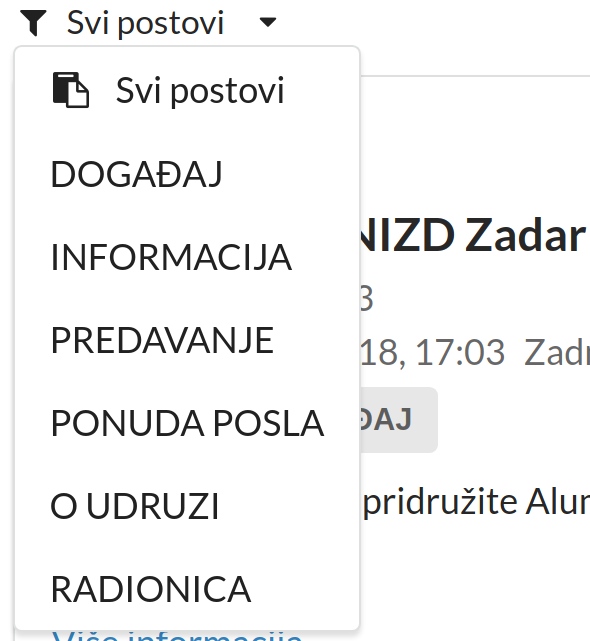
\includegraphics[width=13cm]{slike/filter.png}
	\caption{Padajući izbornik za filtriranje postova}
	\label{fig:filter}
\end{figure}

Postovi mogu biti različitih kategorija, a korisniku sustava često neće biti bitne sve te kategorije. Zbog toga je korisniku omogućeno filtriranje postova po kategorijama putem padajućeg izbornika na vrhu stranice svih postova. Tekst padajućeg izbornika se dinamički mijenja, te se ovisno o tome koja je kategorija izabrana za filtriranje tekst postavi na naziv te kategorije. Osim filtriranja pomoću tog izbornika, filtriranje se može obaviti i odabirom na oznaku kategorije na svakom postu.

\subsection{Pregled posta}

\begin{figure}[H]
	\centering
	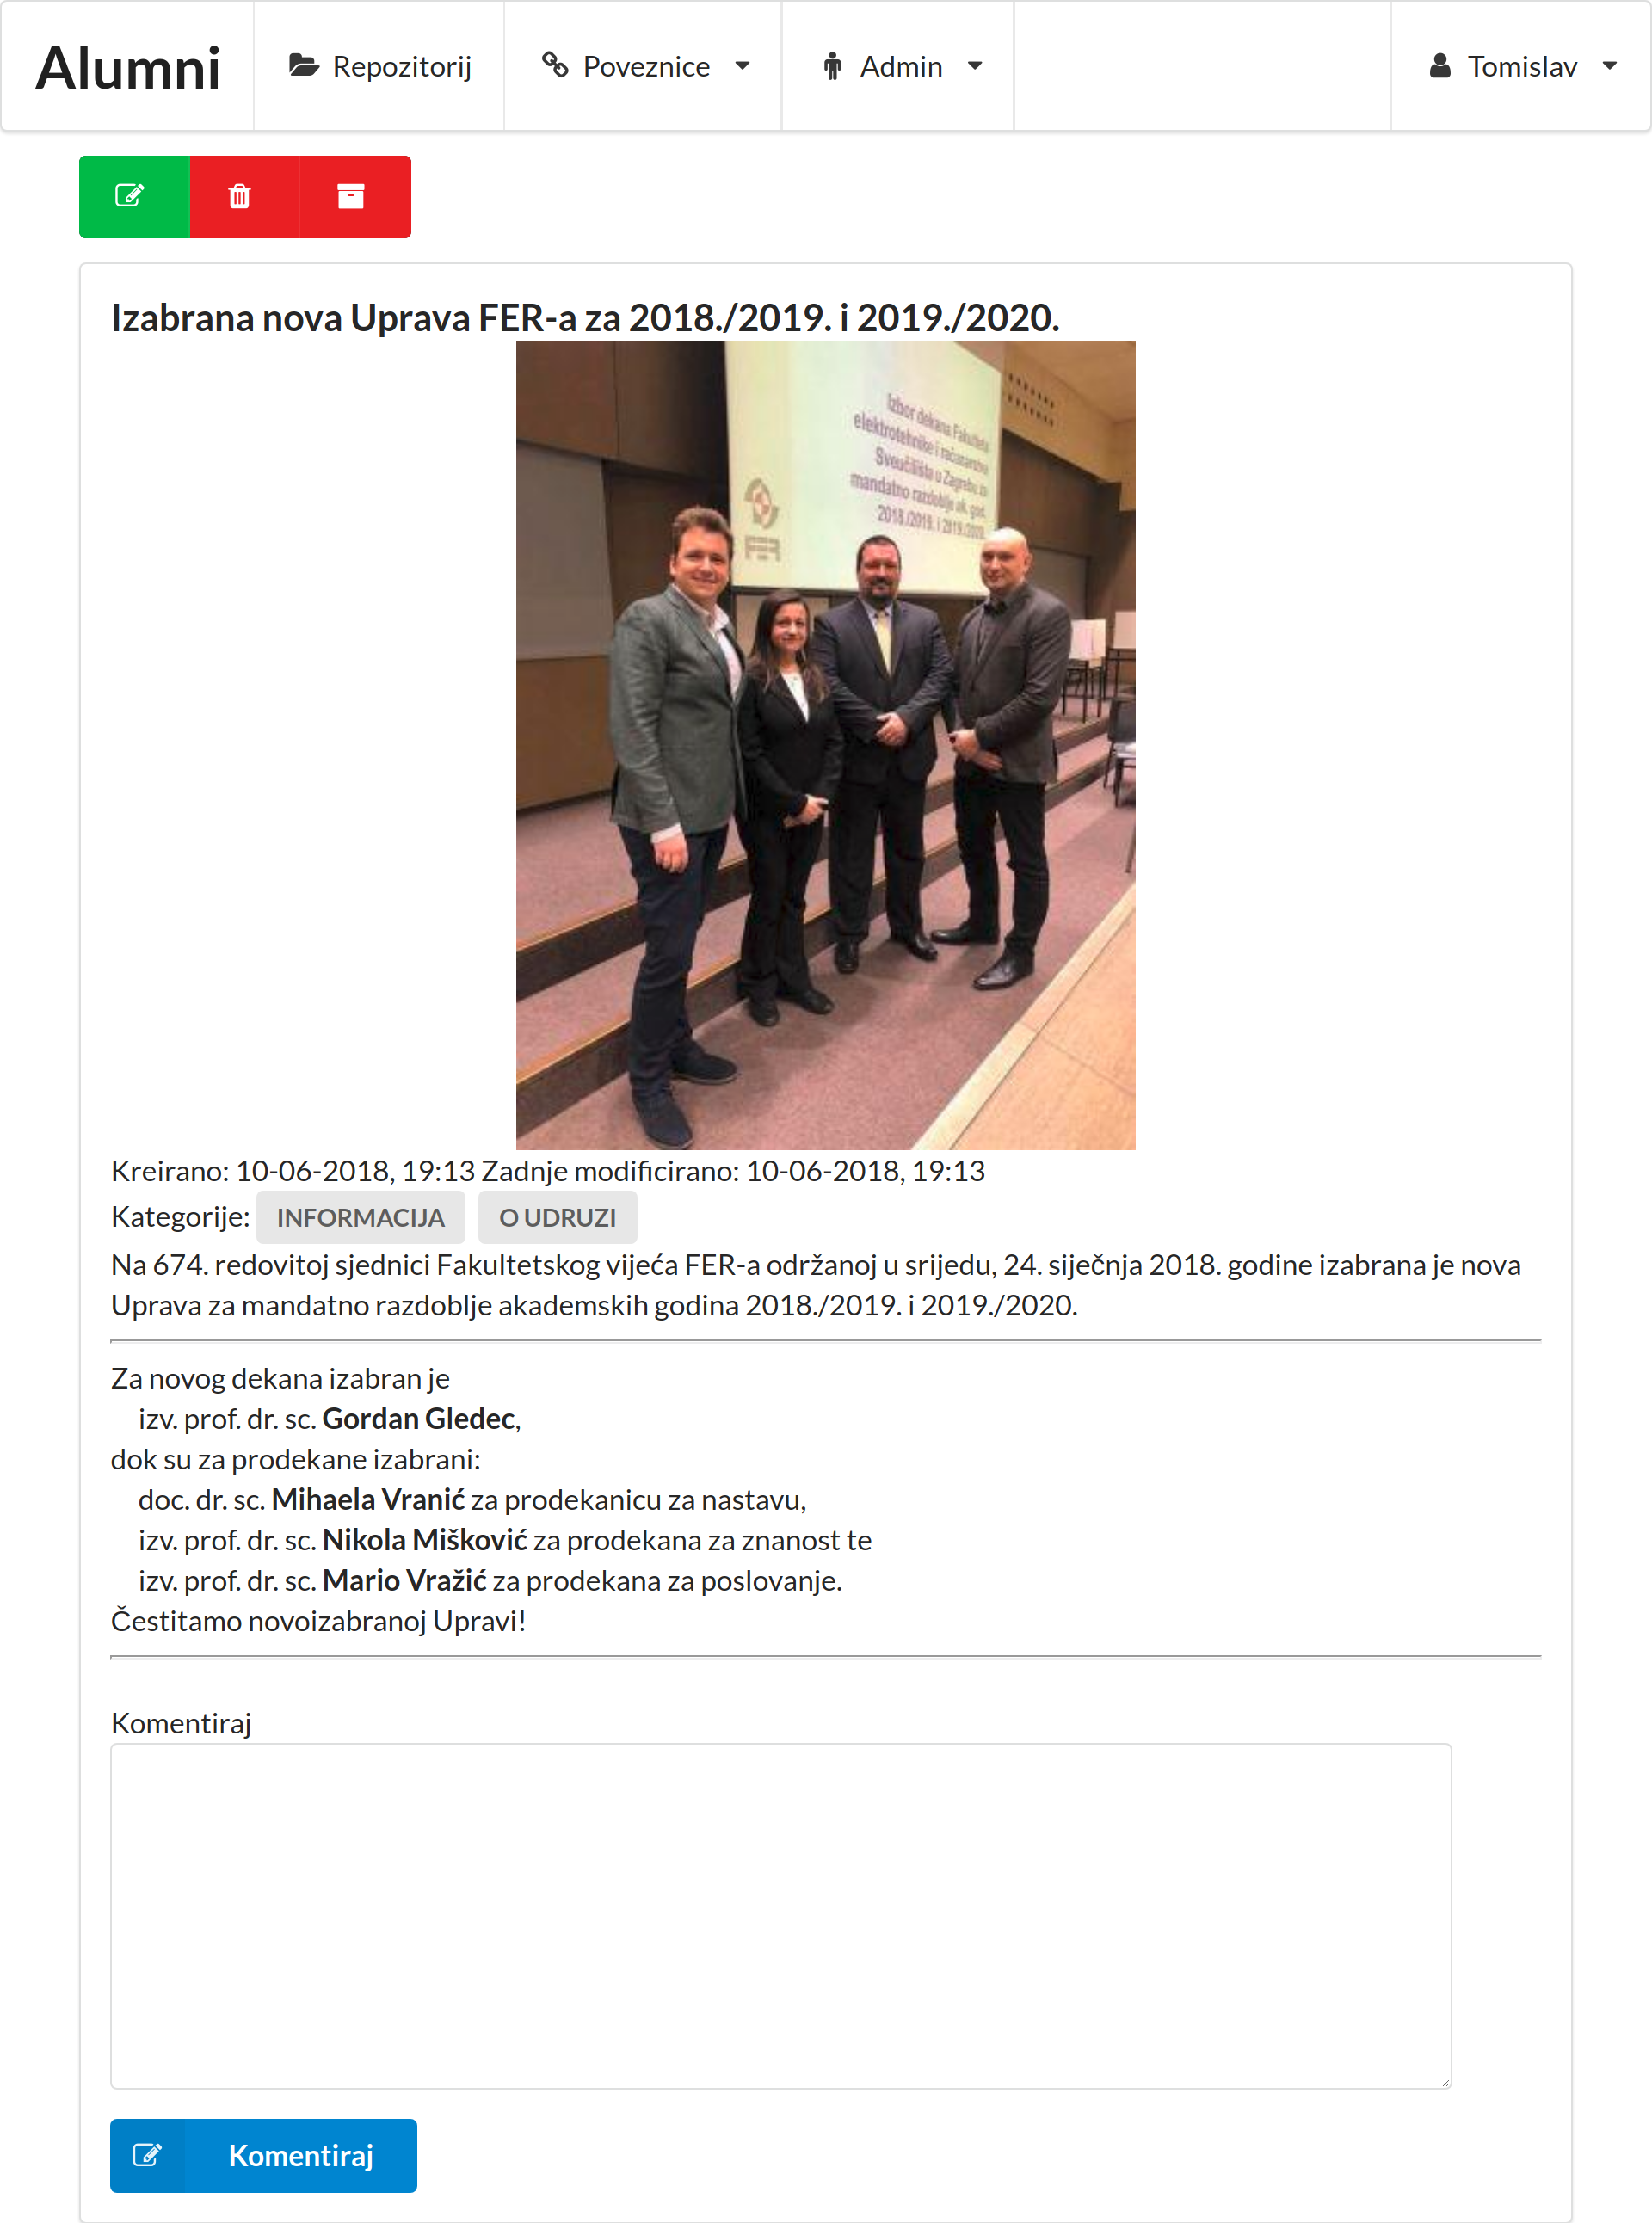
\includegraphics[width=13cm]{slike/post.png}
	\caption{Pregled posta}
	\label{fig:post}
\end{figure}

Odabirom poveznice "Više informacija" ili odabirom naslova posta na stranici pregleda svih postova, dolazi se do stranice za pregled određenog posta gdje se nalazi sve što postoji i na pregledu svih postova, uz dodatan dio gdje se nalazi dugi opis posta.

Također, pri vrhu stranice nalaze se administratorske opcije uređivanja, brisanja te arhiviranja posta.
 
\subsection{Dodavanje novog posta}

\begin{figure}[H]
	\centering
	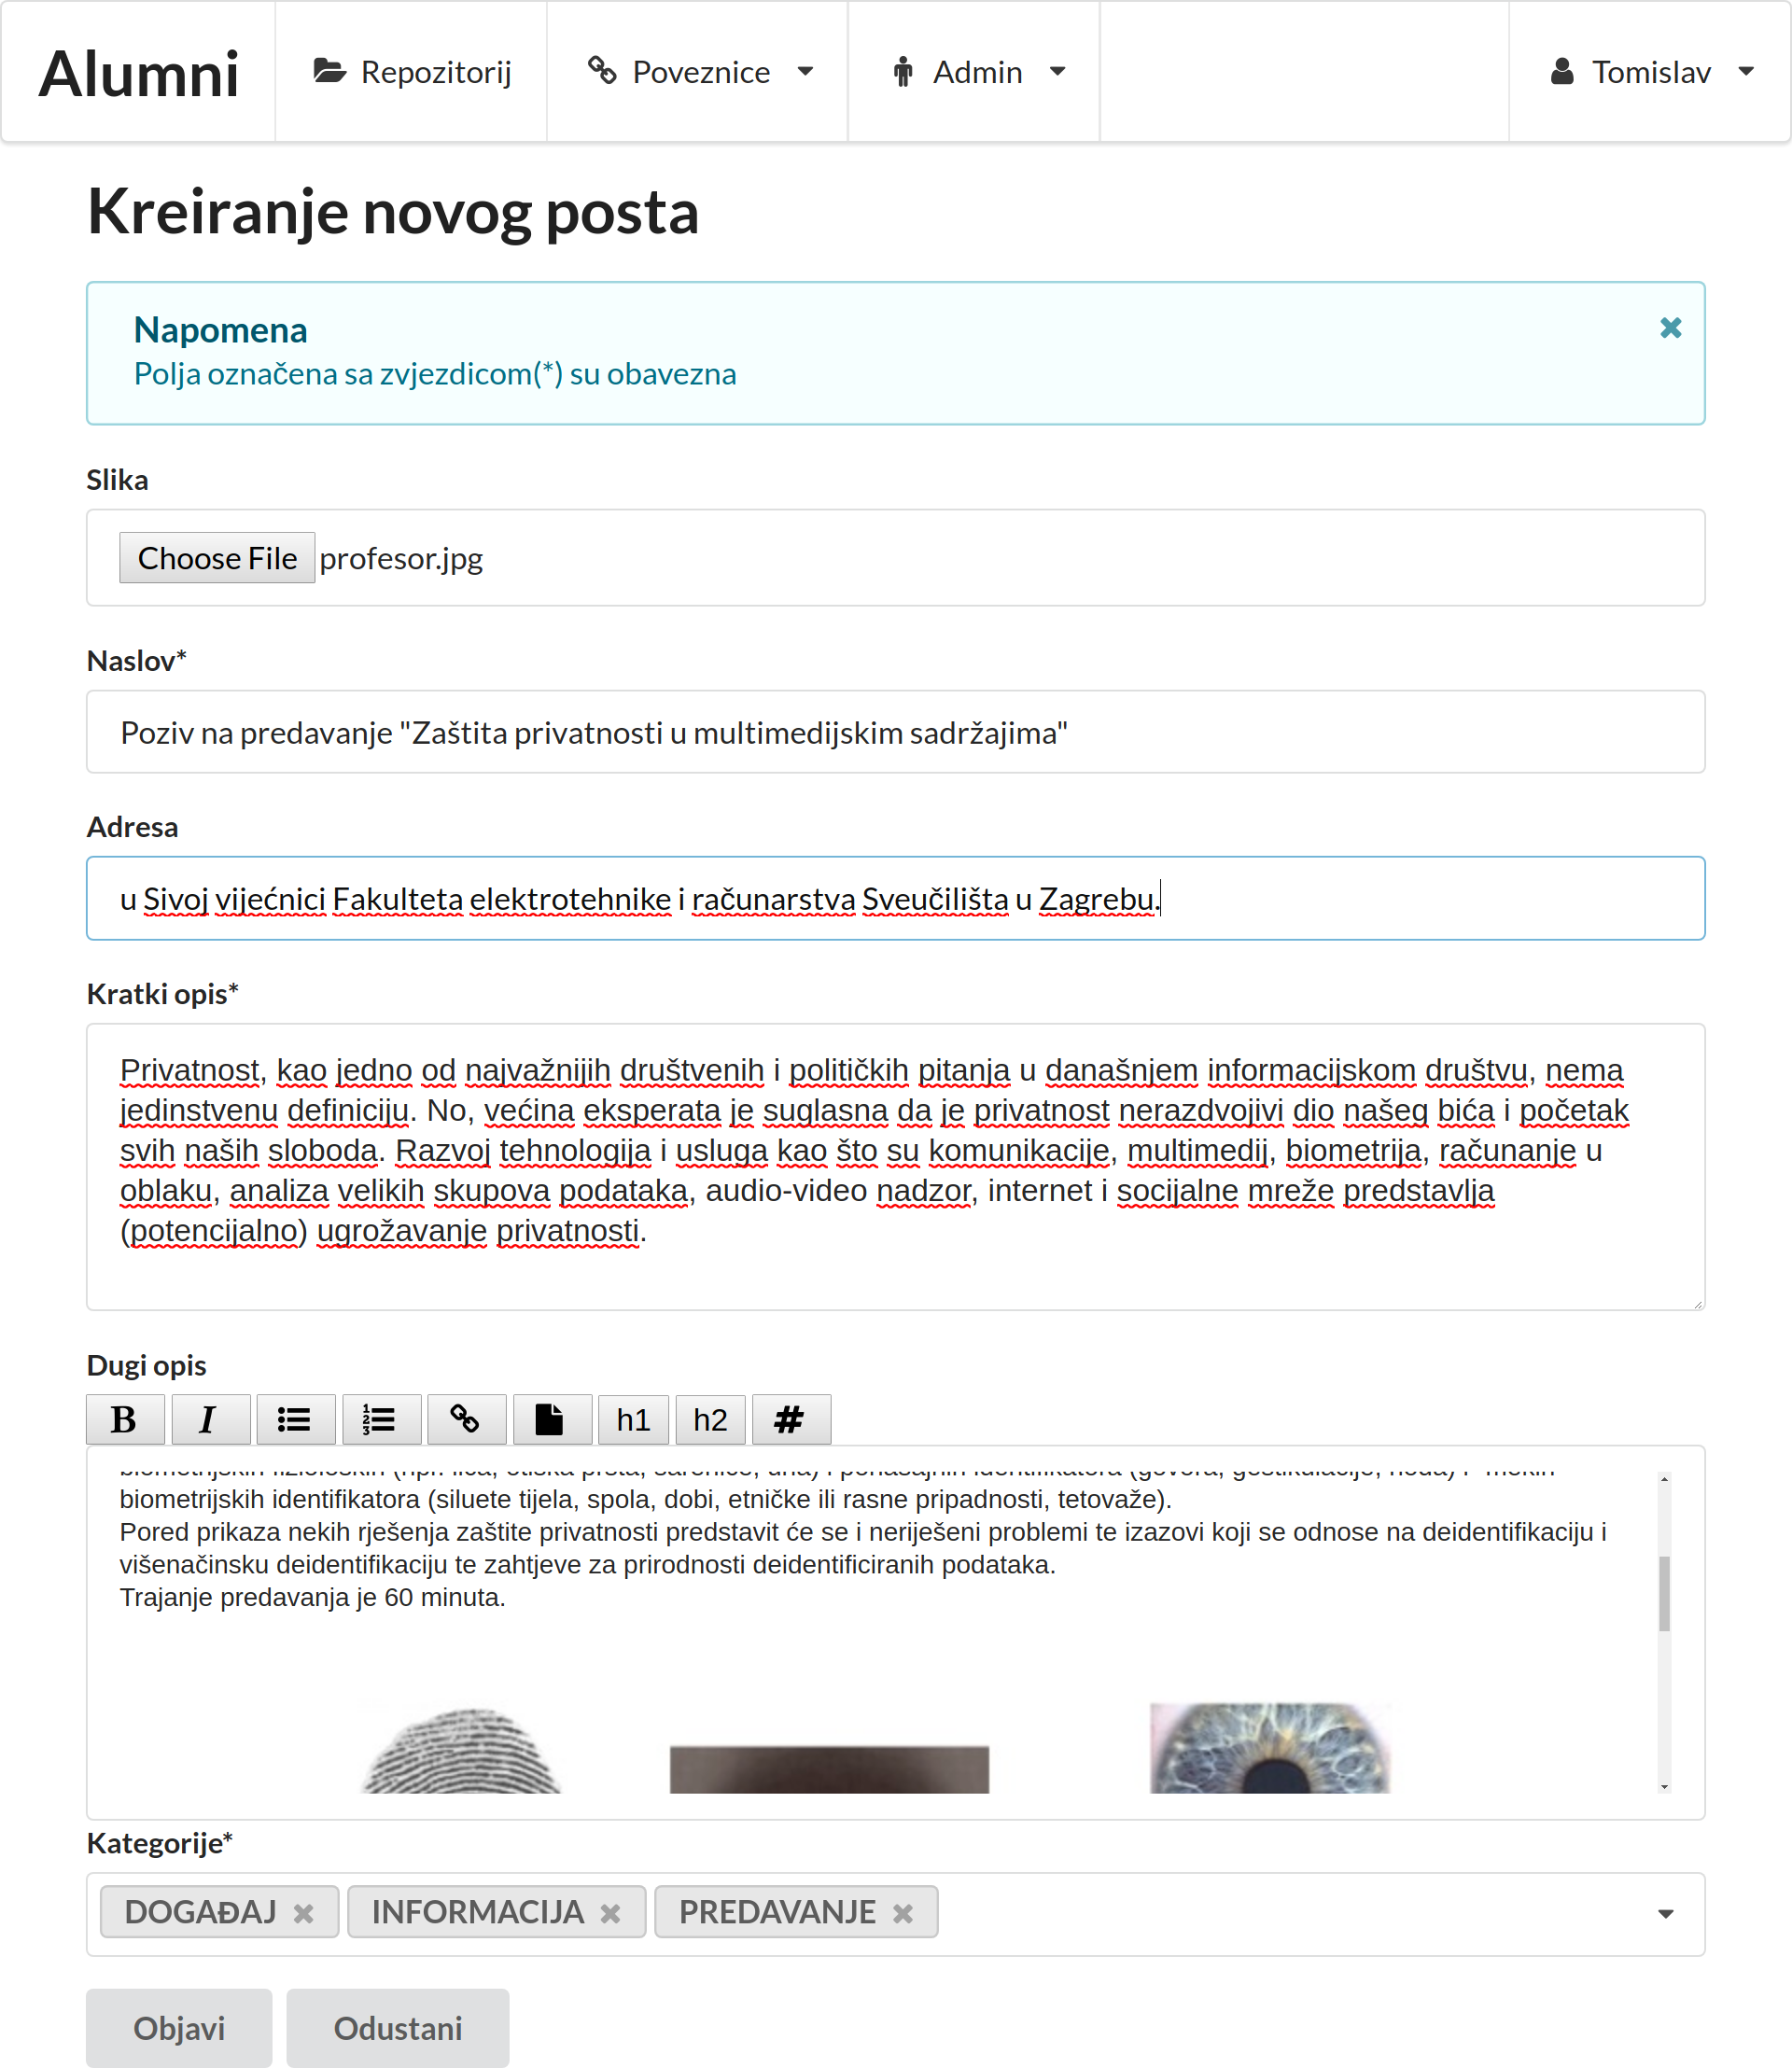
\includegraphics[width=13cm]{slike/novi-post.png}
	\caption{Obrazac za dodavanje novog posta}
	\label{fig:novi-post}
\end{figure}

Do obrasca za dodavanje novog posta dolazi se odabirom opcije "Novi post" u padajućem izborniku "Admin". Dodavanje novog posta zahtijeva upis naslova, kratkog opisa te odabira kategorija postova. Dok su neobavezna polja adresa(lokacija održavanja ako je događaj, dvorana ako je predavanje) i dugi opis posta. Dodavanje dugog opisa posta ostvareno je funkcionalnim uređivačem teksta, zbog administratora koji možda nisu upoznati sa html sintaksom. Kao opcije za uređivanje omogućeno je podebljanje teksta, ukošavanje teksta, izrada neporedane liste, izrada poredane, brojevima označene liste, ubacivanje poveznice, ubacivanje slike, izrada velikog naslova, izrada naslova srednje veličine, te prikaz teksta u html formatu za naprednije korisnike koji žele dodatno uljepšati tekst opcijama koje nisu ponuđene.

\subsection{Uređivanje posta}
Uređivanje posta je ostvareno tako da bude gotovo identično stvaranju novog posta, uz već upisana polja s postojećim podacima.

\subsection{Brisanje posta}
Brisanjem posta brišu se i svi komentari na taj post, a ostvarivo je preko stranice za pregled svih postova ili preko stranice za dotični post koji želimo obrisati.

\subsection{Arhiviranje posta}
Arhiviranje posta je vrlo bitno jer postovi nakon nekog vremena postaju beznačajni, npr. nakon odvijanja događaja o kojem je bio taj post. Ali svejedno ga ne želimo iz nekog razloga obrisati iz sustava jer možda sadrži neku bitnu informaciju, ili čisto radi statistike. Zbog toga postoji funkcionalnost arhiviranja posta koju odrađuje administrator odabirom opcije arhiviranja na pregledu svih postova ili na stranici određenog posta. Ako je post arhiviran, on se više neće prikazivati na pregledu svih postova, nego ćemo ga pronaći na pregledu arhiviranih postova.

\subsection{Pregled arhiviranih postova}

\begin{figure}[H]
	\centering
	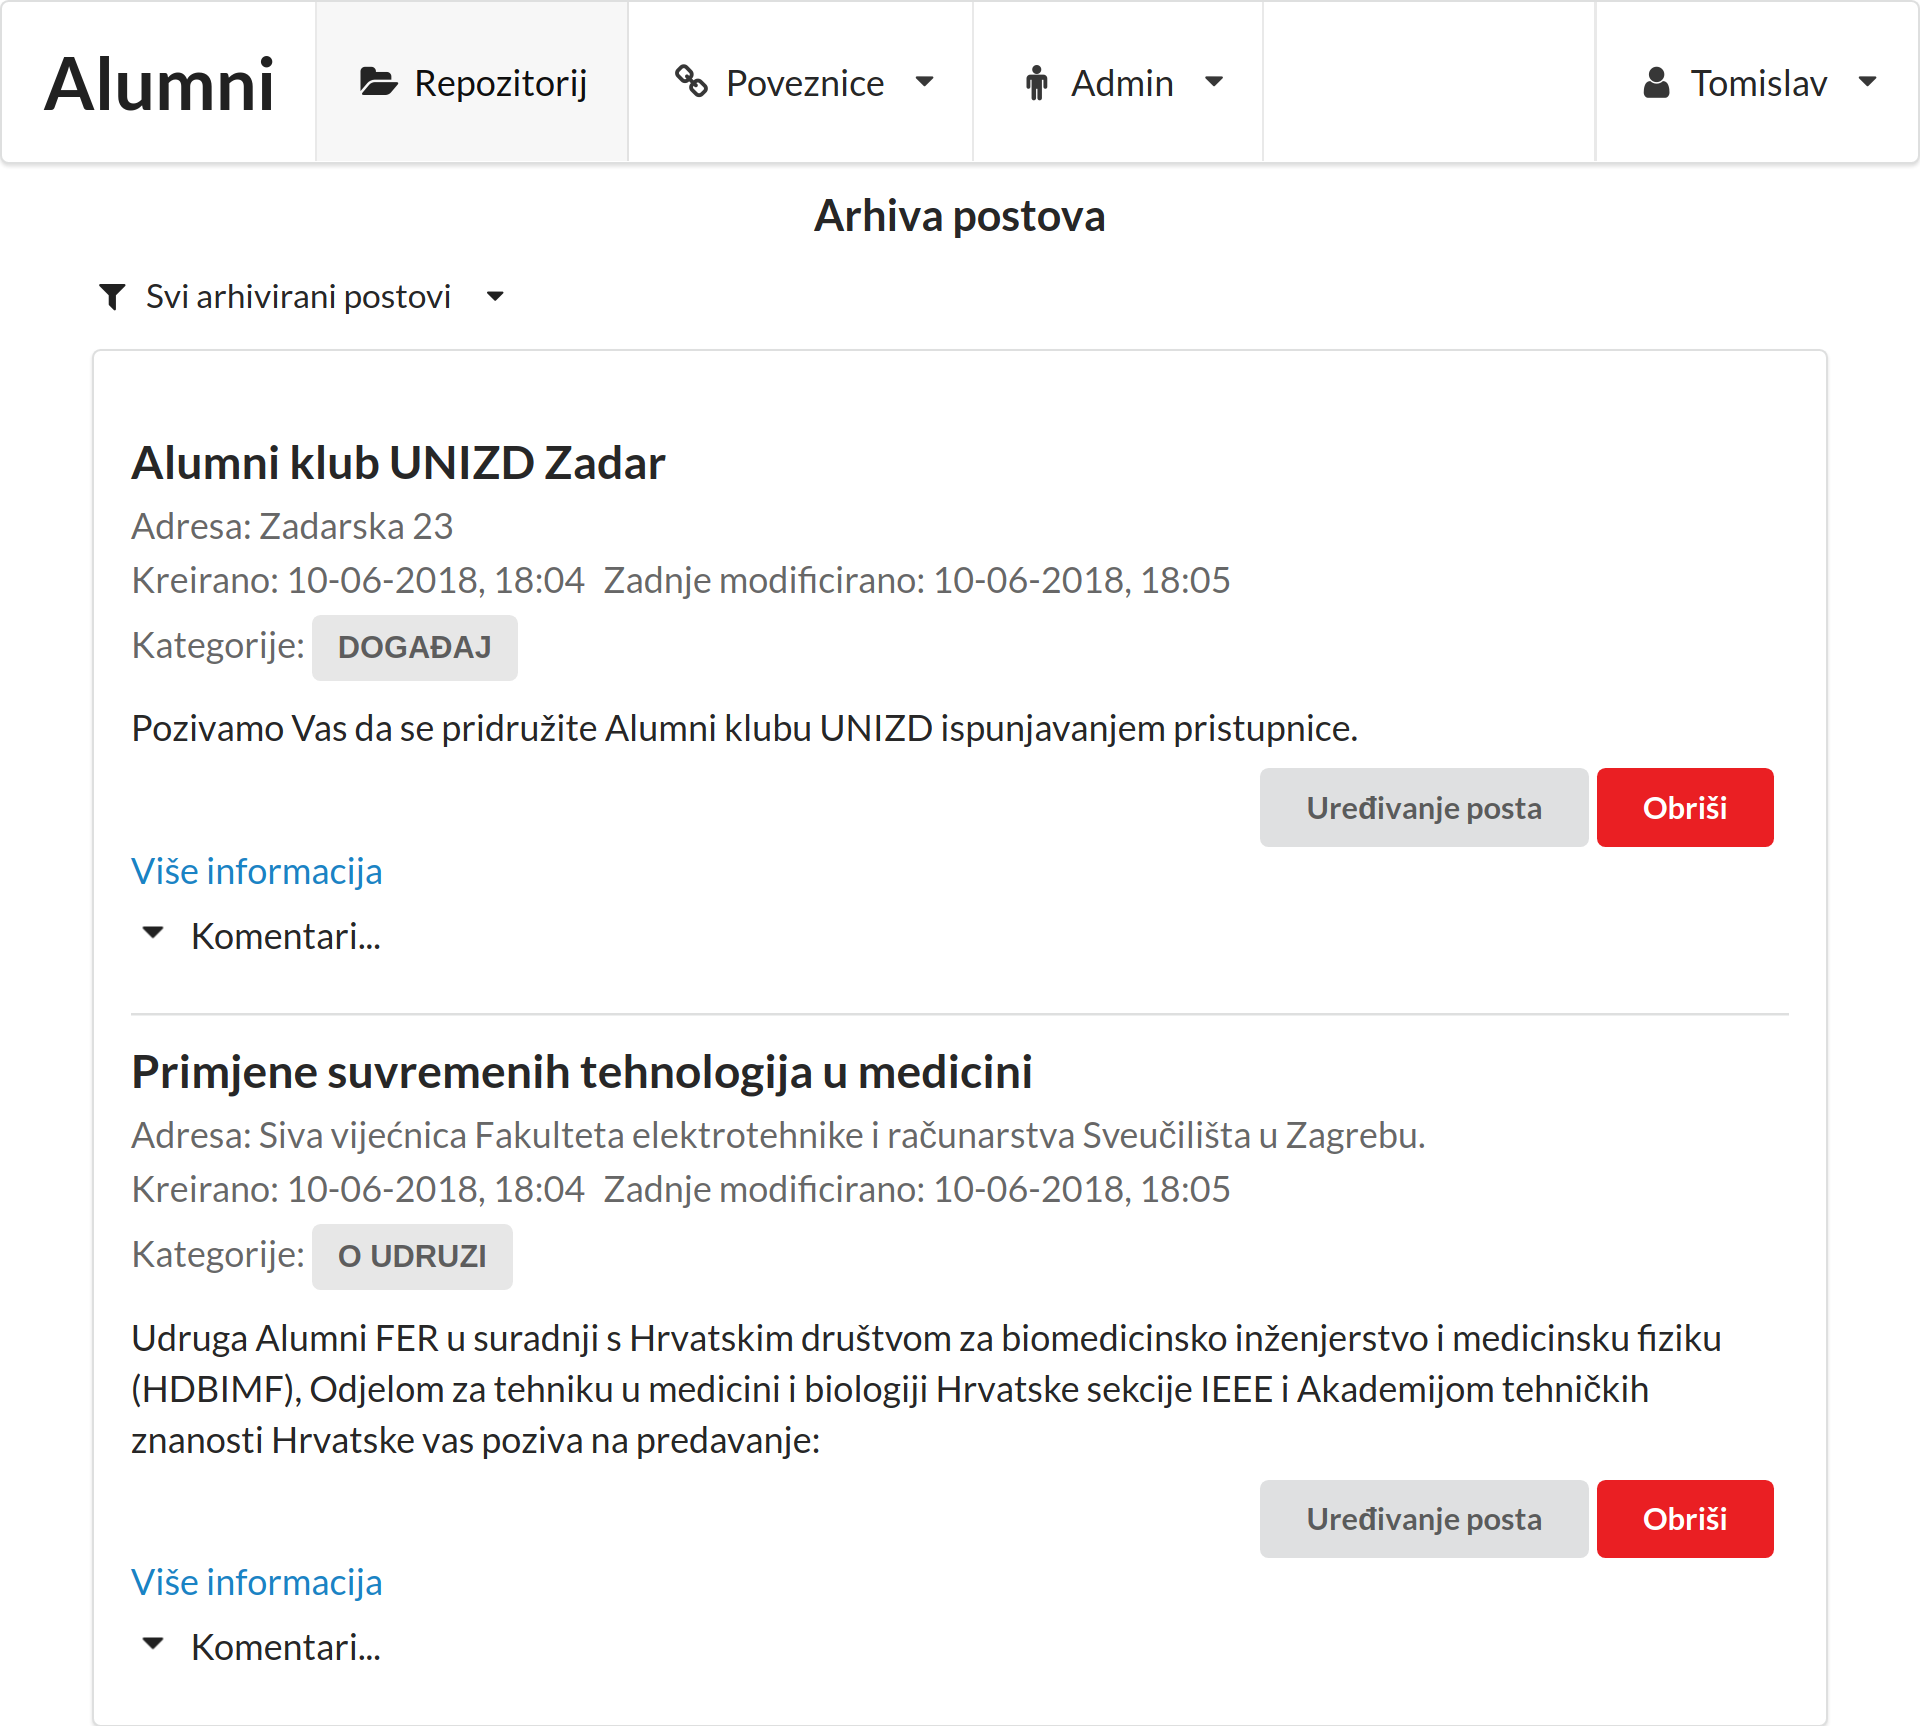
\includegraphics[width=13cm]{slike/arhivirani-postovi.png}
	\caption{Pregled arhiviranih postova}
	\label{fig:arhivirani-postovi}
\end{figure}

Do pregleda arhiviranih postova dolazi se odabirom opcije "Arhiva postova" u padajućem izborniku "Admin" na navigacijskoj traci. Arhiva postova imitira stranicu za prikaz svih postova, te je također omogućeno filtriranje, straničenje, brisanje te uređivanje tih postova.

\subsection{Komentari}

\begin{figure}[H]
	\centering
	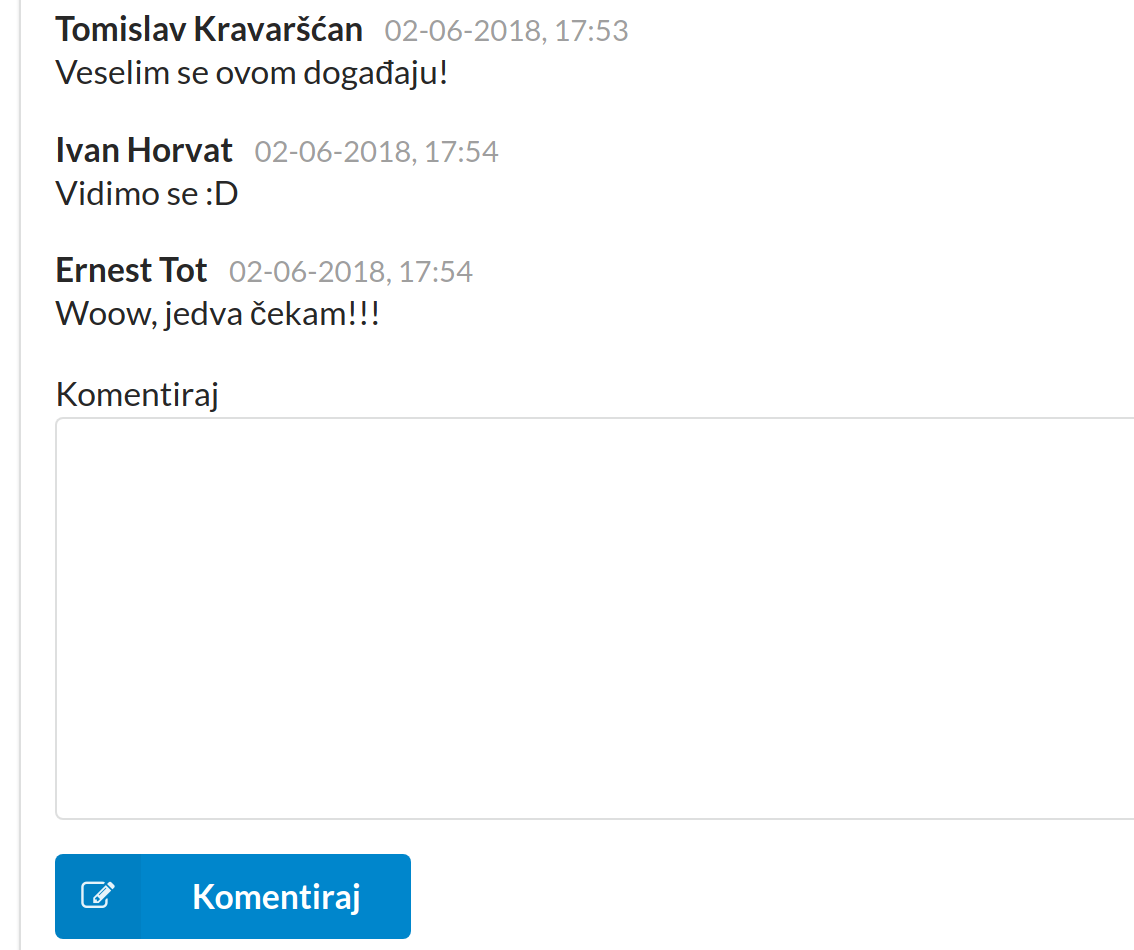
\includegraphics[width=13cm]{slike/komentari.png}
	\caption{Komentari na postu}
	\label{fig:komentari}
\end{figure}

Zbog toga što je ovo stranica za upravljanje zajednicom, vrlo je bitan društveni aspekt te zajednice te je vrlo bitna interakcija korisnika sa sustavom i međusobno. To je ostvareno preko sustava komentara kojim bilo koji prijavljeni korisnik može komentirati postove.

\subsubsection{Dodavanje novog komentara}

Čim je korisnik prijavljen na sustav, može komentirati na post iz pregleda svih postova, odabirom opcije "Komentari...", upisivanjem komentara u obrazac i pritiskom gumba za komentiranje. Prilikom komentiranja postoji provjera da li komentar postoji, odnosno nije moguće izraditi prazan komentar. Za svaki komentar je u pregledu komentara postova prikazan autor tog komentara, odnosno njegovo ime i prezime, datum objave tog komentara, te sadržaj komentara.

\subsubsection{Brisanje komentara}
Korisnici imaju mogućnost komentiranja bilo čega, pa ti komentari često mogu biti zlonamjerni ili neprimjereni. Zato je administratoru omogućeno brisanje komentara pomoću ikonice smeća pored datuma komentara.

\section{Sustav pretplata}
Korisnici često propuste neke važne obavijesti na stranicama ako redovno ne posjećuju te stranice. Zbog toga postoji sustav pretplata pomoću kojeg se korisnik pretplati na željene kategorije postova. Od tog trenutka nadalje, korisnik prilikom svake objave posta koji sadrži kategoriju na koju je korisnik pretplaćen, dobiva obavijest na email.

\subsection{Dodavanje i ažuriranje pretplata}

\begin{figure}[H]
	\centering
	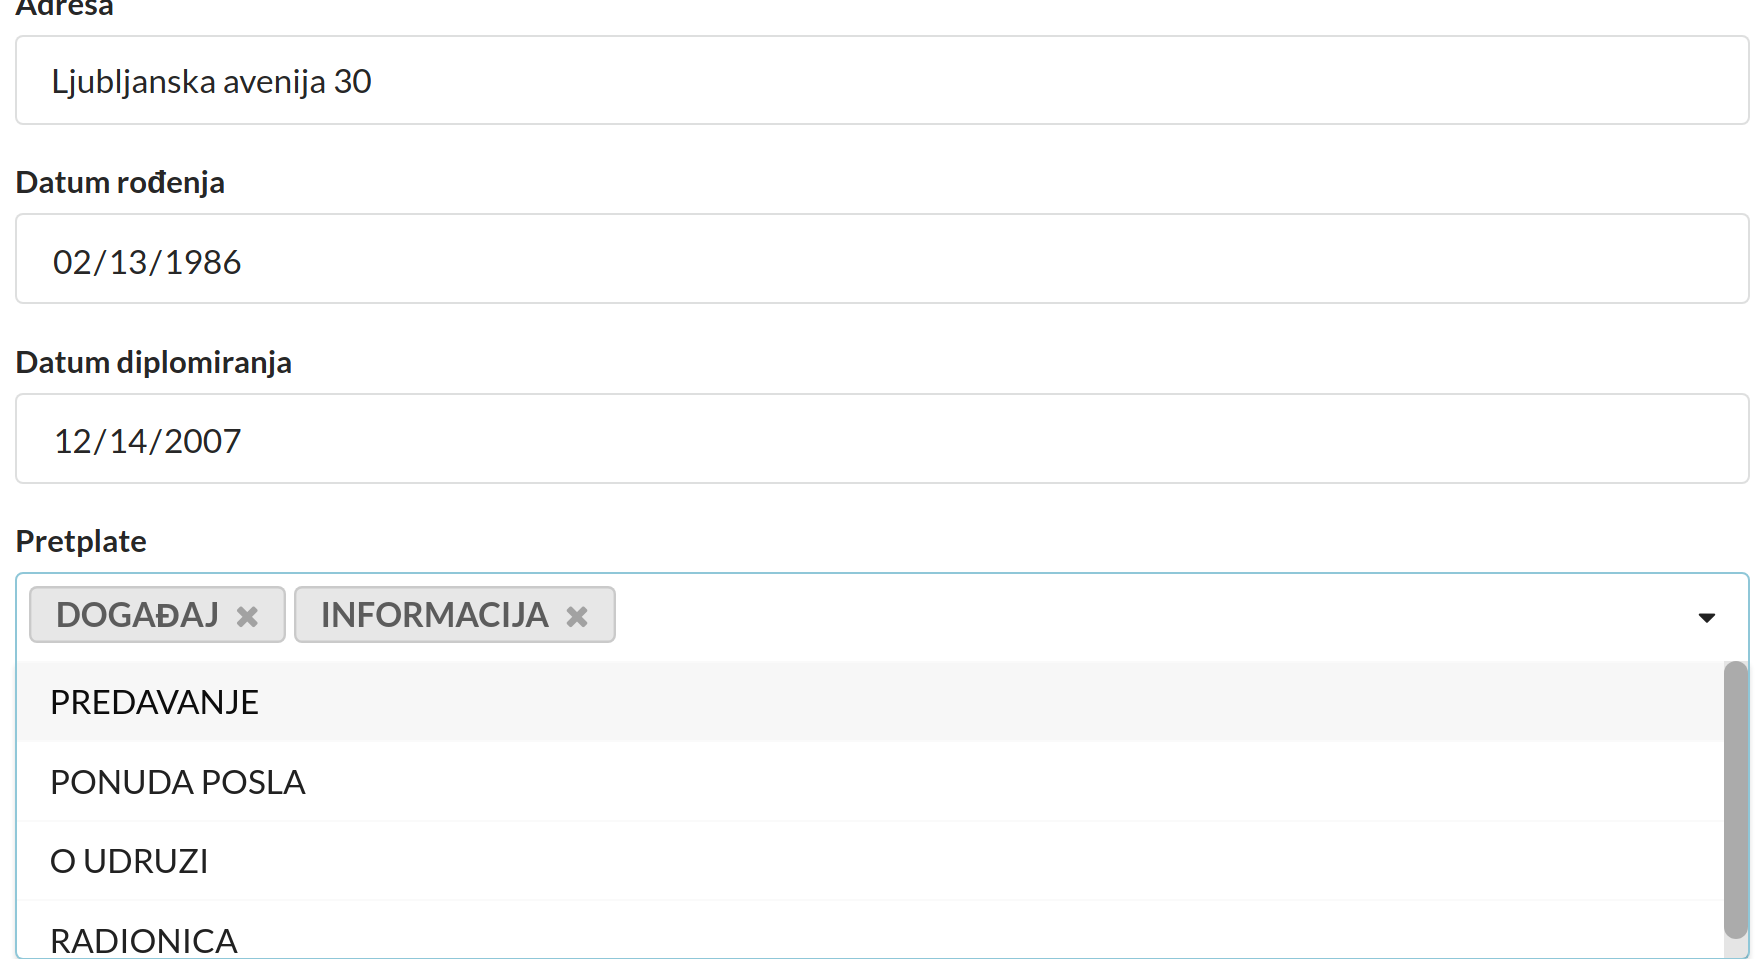
\includegraphics[width=13cm]{slike/pretplate.png}
	\caption{Dodavanje pretplata na obrascu za uređivanje korisnika}
	\label{fig:pretplate}
\end{figure}

Uređivanje pretplata ostvareno je u sklopu uređivanja korisničkog računa, pri dnu obrasca. Korisnik se pomoću više-odabirnog padajućeg izbornika može pretplatiti na određene kategorije postova. Na taj isti način mogu se i ukloniti pretplate. Korisnik ne mora nužno biti pretplaćen na bilo koju kategoriju. Ako je korisnik pretplaćen na neke kategorije, to je vidljivo na pregledu njegovog računa.

\subsection{Slanje pošte prilikom dodavanja novog posta}

\begin{figure}[H]
	\centering
	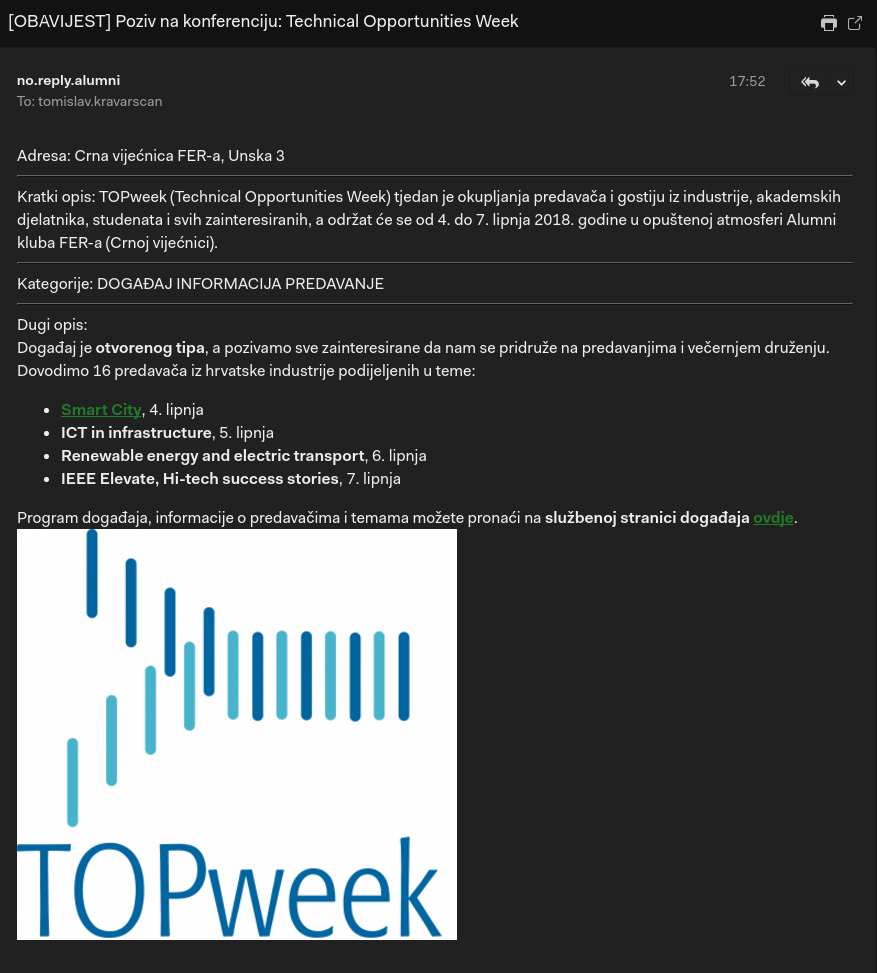
\includegraphics[width=13cm]{slike/mail.png}
	\caption{Izgled pošte obavijesti} 
	\label{fig:mail}
\end{figure}

Kada administrator na stranici izradi novi post, automatski se svim korisnicima koji su pretplaćeni na kategorije koje sadrži taj post šalje mail sa cjelokupnim sadržajem tog posta, kao što je vidljivo na slici. 


\chapter{Zaključak}
Zaključak.

\bibliography{literatura}
\bibliographystyle{fer}

\begin{sazetak}
	Sažetak na hrvatskom jeziku.
			
	\kljucnerijeci{Ključne riječi, odvojene zarezima.}
\end{sazetak}

% TODO: Navedite naslov na engleskom jeziku.
\engtitle{Title}
\begin{abstract}
	Abstract.
			
	\keywords{Keywords.}
\end{abstract}

\end{document}
